%% Submissions for peer-review must enable line-numbering
%% using the lineno option in the \documentclass command.
%%
%% Preprints and camera-ready submissions do not need
%% line numbers, and should have this option removed.
%%
%% Please note that the line numbering option requires
%% version 1.1 or newer of the wlpeerj.cls file, and
%% the corresponding author info requires v1.2

\documentclass[fleqn,10pt,lineno]{wlpeerj} % for journal submissions

% ZNK -- Adding headers for pandoc

\setlength{\emergencystretch}{3em}
\providecommand{\tightlist}{
\setlength{\itemsep}{0pt}\setlength{\parskip}{0pt}}
\usepackage{lipsum}
\usepackage[unicode=true]{hyperref}
\usepackage{longtable}


\usepackage{lipsum} \usepackage{textcomp, rotating}
\usepackage[normalem]{ulem}

\title{Detecting the impact of land cover change on observed rainfall.}

\author[1]{Chun X. Liang}

\author[1]{Floris F. van Ogtrop}

\author[1]{R. Willem Vervoort}

\corrauthor[1]{R. Willem Vervoort}{\href{mailto:willem.vervoort@sydney.edu.au}{\nolinkurl{willem.vervoort@sydney.edu.au}}}

\affil[1]{School of Life and Environmental Sciences, Sydney Institute of
Agriculture, The University of Sydney, New South Wales, Australia.}


%
% \author[1]{First Author}
% \author[2]{Second Author}
% \affil[1]{Address of first author}
% \affil[2]{Address of second author}
% \corrauthor[1]{First Author}{f.author@email.com}

% 

\begin{abstract}
Analysis of observational data to pinpoint impact of land cover change
on local rainfall is difficult due to multiple environmental factors
that cannot be strictly controlled. In this study we use a statistical
approach to identify the relationship between removal of tree cover and
rainfall with data from best available sources for two large areas in
Australia. Gridded rainfall data between 1979 and 2015 was used for the
areas, while large scale (exogenous) effects were represented by mean
rainfall across a much larger area and climatic indicators, such as
Southern Oscillation Index and Indian Ocean Dipole. Both generalised
additive modelling and step trend tests were used for the analysis. For
a region in south central Queensland, the reported change in tree
clearing between 2002 - 2005 did not result in strong statistically
significant precipitation changes. On the other hand, results from a
bushfire affected region on the border of New South Wales and Victoria
suggests significant changes in the rainfall due to changes in tree
cover. This indicates the method works better when an abrupt change in
the data can be clearly identified. The results from the step trend test
also mainly identified a positive relationship between the tree cover
and the rainfall at p \textless{} 0.1 at the NSW/Victoria region. High
rainfall variability and possible regrowth could have impacted the
results in the Queensland region.
% Dummy abstract text. Dummy abstract text. Dummy abstract text. Dummy abstract text. Dummy abstract text. Dummy abstract text. Dummy abstract text. Dummy abstract text. Dummy abstract text. Dummy abstract text. Dummy abstract text.
\end{abstract}

\usepackage{amsthm}
\newtheorem{theorem}{Theorem}[section]
\newtheorem{lemma}{Lemma}[section]
\theoremstyle{definition}
\newtheorem{definition}{Definition}[section]
\newtheorem{corollary}{Corollary}[section]
\newtheorem{proposition}{Proposition}[section]
\theoremstyle{definition}
\newtheorem{example}{Example}[section]
\theoremstyle{definition}
\newtheorem{exercise}{Exercise}[section]
\theoremstyle{remark}
\newtheorem*{remark}{Remark}
\newtheorem*{solution}{Solution}
\begin{document}

\flushbottom
\maketitle
\thispagestyle{empty}

\section*{Introduction}\label{introduction}
\addcontentsline{toc}{section}{Introduction}

Land use and land cover changes can lead to changes in the local
climate. Empirical and modelling studies have found that cloud types and
rainfall are correlated to large scale vegetation cover changes, such as
deforestation in the Amazon and in the Sahel (Chagnon \& Bras, 2005;
Wang et al., 2009; Pinto et al., 2009; Mei \& Wang, 2010; Kucharski,
Zeng \& Kalnay, 2013; Pitman \& Lorenz, 2016) and afforestation in south
Israel (Otterman et al., 1990; Ben-Gai et al., 1998). Using airborne
measurements in Western Australia, Junkermann et al. (2009) showed a
significantly higher level of aerosols over an agricultural area
compared to an adjacent area with natural vegetation. They suggested
that a modification of aerosol concentrations due to deforestation could
have contributed to a reduction of local rainfall, as more, but smaller
rain droplets were observed. Nair et al. (2011) reported from the Bunny
Fence Experiment in Western Australia that local land use change altered
the synoptic west coast trough dynamics and surface roughness, and this
resulted in an observed rainfall decrease. Maximum temperatures were
also found to be sensitive to land cover change in eastern Australia
(McAlpine et al., 2007).

Overall the number of empirical studies analyzing changes to rainfall
due to land cover change from observational data is limited. Most of the
studies mentioned previously were either model simulations, or
comparisons of modelled data with observations. This is because there
are some fundamental experimental difficulties in both space (where does
evaporated water reappear as rainfall?) and time (how much time does it
take for land cover change effects to appear or disappear?). In
addition, in many areas across the globe, rainfall variability is
related to a complex set of interactions (outlined below), of which land
use change might only be a minor component.

Locally, and on a shorter, daily time scale, there are two main sources
that generate rainfall: moisture from advective atmospheric transport;
and local evapotranspiration (Eltahir \& Bras, 1996; Bosilovich \&
Chern, 2006; Dirmeyer, Brubaker \& DelSole, 2009; Gimeno et al., 2010).
The local evapotranspiration component is the component considered to be
affected by land use change (Eltahir \& Bras, 1996). According to
Trenberth (1999), the contribution of advective moisture partially
depends on the availability of external moisture and atmospheric
transport. On the longer time scale, such as monthly and annually, large
scale atmospheric dynamics are affected by large scale climate drivers.
For example, many studies have reported significant relationships
between rainfall in large parts of Australia and the El Niño-Southern
Oscillation (ENSO) (Verdon et al., 2004; Risbey et al., 2009; Speer,
Leslie \& Fierro, 2011). In contrast, local ET is determined by local
land surface characteristics, which influence local scale atmospheric
dynamics and hence the amount of rainfall, including contribution from
both main sources.

Although climate drivers demonstrate some capability to predict
Australian rainfall, there is still a large amount of unexplained
variance. Westra \& Sharma (2010) pointed out that models based on
global sea surface temperature anomalies can only predict up to 14.7\%
of annual precipitation variance. More generally, some of the remaining
variance could be due to land surface processes as suggested in studies
predicting local rainfall (e.g. Ma et al., 2011; Zeng et al., 2012;
Pitman \& Lorenz, 2016; Saha, Dirmeyer \& Chase, 2016). However, most
are based on modelling experiments and few empirical observational
studies have been reported. However, Pitman et al. (2004) found a good
match between observations and simulated rainfall changes in southwest
Western Australia, forced by land cover change. Timbal \& Arblaster
(2006) were able to reproduce the rainfall decline in south west
Australia by including land cover influence. In addition, local land use
change might not be a primary, but is likely to be a secondary cause of
rainfall change (Nicholls, 2006).

Therefore, the aim of this study is to use a statistical approach on
rainfall data at regional scales to investigate the cause and effect
relationship between land cover change and local rainfall, which is
demonstrated in many modelling studies. More specifically, we
hypothesize that a step change in land cover on the surface will cause a
step change in the rainfall. To demonstrate this we study changes in
observed rainfall over time at a Queensland and NSW/Victoria location
where there are possible step changes in land cover change due to land
clearing and bush fires. The methodology uses statistical approaches to
identify changes in rainfall, which are subsequently associated with
land cover change through spatial comparison.

In this paper, after this section (the introduction), section 2 covers
the case study areas and the observed land use change. Section 3
describes the data used in the study in more detail. Section 4 details
the statistical methods and the underlying assumptions related to the
modelling approach, Section 5 gives the results, which are further
discussed in section 6 and finally section 7 offers the conclusions.

\section{Study regions and tree cover
change}\label{study-regions-and-tree-cover-change}

In Australia, significant tree cover change has mainly occurred in the
north east and south east of the continent, as well as in the southwest
of Western Australia. According to the National Dynamic Land Cover
Dataset (DLCD) (Lymburner et al., 2010), most of these areas have
experienced decreases in the Enhanced Vegetation Index (EVI) post 2000,
as derived from satellite data. As an index for vegetation greenness,
the decreasing values of EVI indicate lower biomass over time in the
tree cover regions. The possible EVI reduction might be due to land
clearing, bush fires or drought.

\begin{figure}
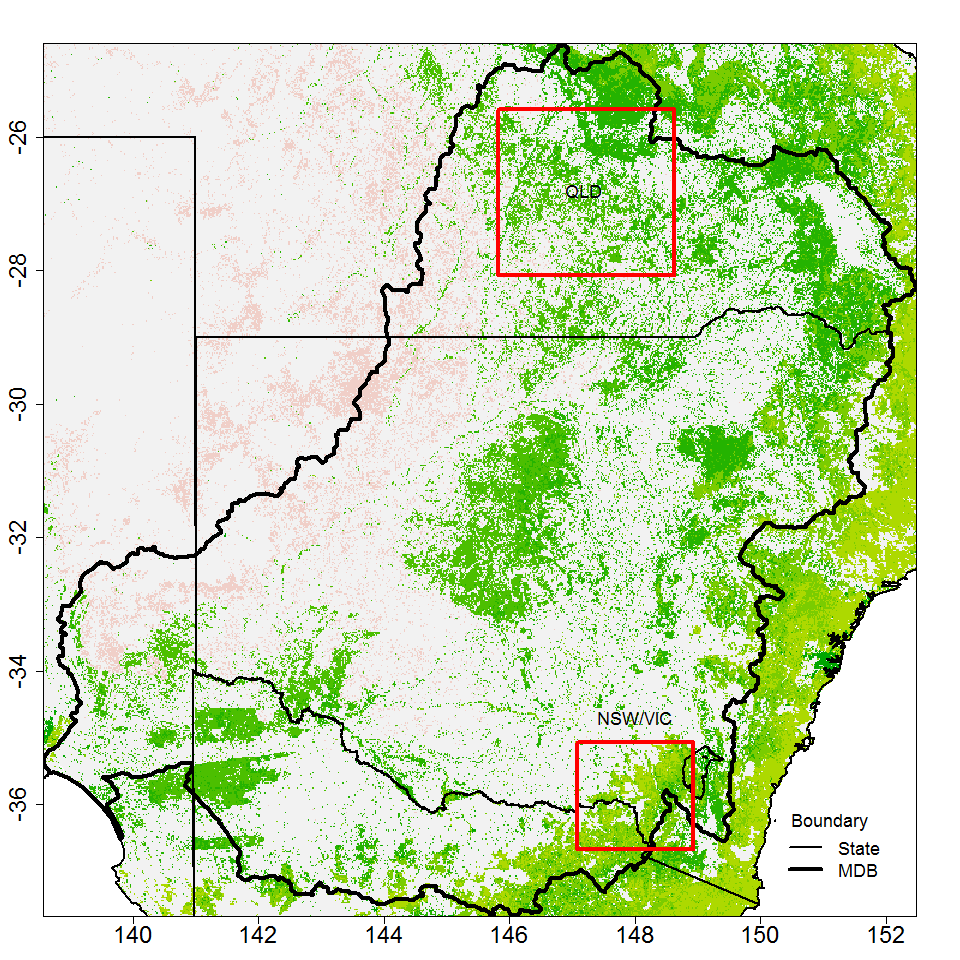
\includegraphics[width=0.9\linewidth]{figures/Fig1} \caption{Selected study regions are highlighted by red rectangles in the main map (the red rectangle in the insert indicates the location of the main map). The types of tree cover in 2008 from the DLCD product is shown at the background. In site 1 (the QLD region), the tree cover is mostly sparse. In site 2 (the NSW/VIC region), many areas have open or close forest where the tree cover is denser.}\label{fig:selreg}
\end{figure}

Two regions were selected where significant tree cover change since 2000
was reported. The first region is located in south central Queensland
(QLD) partly covering the north of the Murray Darling Basin (MDB) (site
1 in Figure \ref{fig:selreg}). High rates of land clearing have been
reported in this region during the early 2000s (Department of Natural
Resources and Water, 2007). The second study region is located at the
border of New South Wales and Victoria (NSW/VIC), and includes the Snowy
Mountain ranges (site 2 in Figure \ref{fig:selreg}). Severe bush fires
occurred in this area in early 2003 (see Figure \ref{fig:bushfire}). The
2003 bush fires were the largest in the last 60 years (The State
Government of Victoria, 2011). Two thirds of Kosciuszko national park
was heavily burned and regrowth was suggested to be slow due to drought
and cold conditions (ABC News, 2003), and the type of species in this
region. However, in the longer term, after an early high transpiration
period a recovery of pre-fire evapotranspiration would be expected
(Kuczera, 1987). For the purpose of this study, significant tree cover
loss has happened in both study areas in the last decade, either
permanently or temporarily.

\begin{figure}
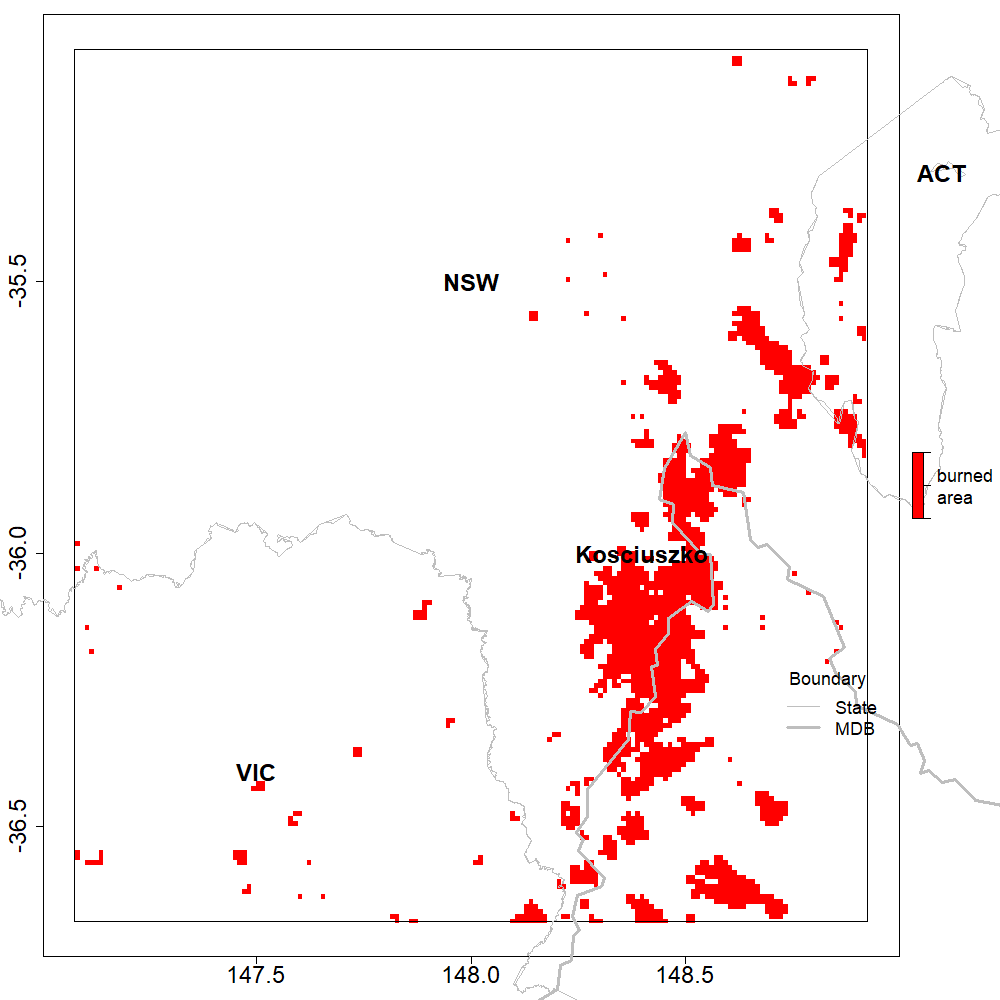
\includegraphics[width=0.9\linewidth]{figures/Fig2} \caption{Location of bushfires occurring in January 2003, in and around the NSW/VIC study region, as shown by the red pixels. The map shows the large area in the Kosciuszko national park that has been burned. Some locations in the southwest of the Australian Capital Territory (ACT) have also experienced intensive bushfires.}\label{fig:bushfire}
\end{figure}

The two regions have different characteristics. The QLD region is
partially grassland and subtropical, while the NSW/VIC region is mainly
within the temperate zone, under the Köppen classification. According
to Australian Bureau of Meteorology (BoM), the NSW/VIC region receives
1000 - 2000 mm rainfall annually, which is more than double the annual
rainfall in the QLD region. Evapotranspiration is similar in both
regions. Marine moisture and orographic effects are likely to be the
main contributors to rainfall in the southeast mountain areas of the
NSW/VIC region.

The land use and land cover characteristics in the two regions are also
different. In the Queensland region, the tree cover is sparse over most
of the area. The MODIS satellite tree cover data (discussed in more
detail in section 3) shows that tree cover in this region is generally
below 20\% of total ground area. Grazing is the main activity in this
region, with over 90\% of land used by the grazing industry (ABARES,
2010). Our starting assumption is that the main cause of the EVI decline
over large part of the region is due to land clearing. Tree cover has
been cleared at a massive scale over the last decade, especially during
2002 - 2004. The reports from the Queensland Statewide Land Cover and
Trees Study (SLATS) (e.g. Department of Natural Resources and Mines,
2005; Department of Science, Information Technology and Innovation,
2017) were used to investigate the time and location of the land
clearing in the QLD region.

The Kosciuszko national park is within the NSW/VIC region. Here tree
cover is denser with open or even closed forest (the tree cover
distribution is bimodal at 10 - 20\% and 60 - 70\%). The dominant
species in the alpine area are Snow Gum (\emph{Eucalyptus
Pauciflora})and large stand species such as Alpine Ash (\emph{Eucalyptus
delegatensis}) and Mountain Gum (\emph{Eucalyptus dalrympleana}) in the
sub-alpine area. These trees can reach a great height but they take long
time to grow. For example, Alpine Ash (\emph{Eucalyptus delegatensis})
would need about 20 years to mature (40 - 45 m, Buckley et al. (2012)).
This region is vulnerable to fires and drought, however land clearing is
not a major issue. The MODIS burned area product, MCD45A1 (Roy, Lewis \&
Justice, 2002; Roy et al., 2005, 2008), was used to locate bush fires
areas in the NSW/VIC region, with a grid resolution of 500 m. MCD45A1
provides monthly burning information on all pixels, which helps to
pinpoint an abrupt event.

Due to the difference in nature of the land cover change in the two
regions, the post-change vegetation status is hypothesized to be
different as well (see Figure \ref{fig:figure3-tc-simple}).

\begin{figure}
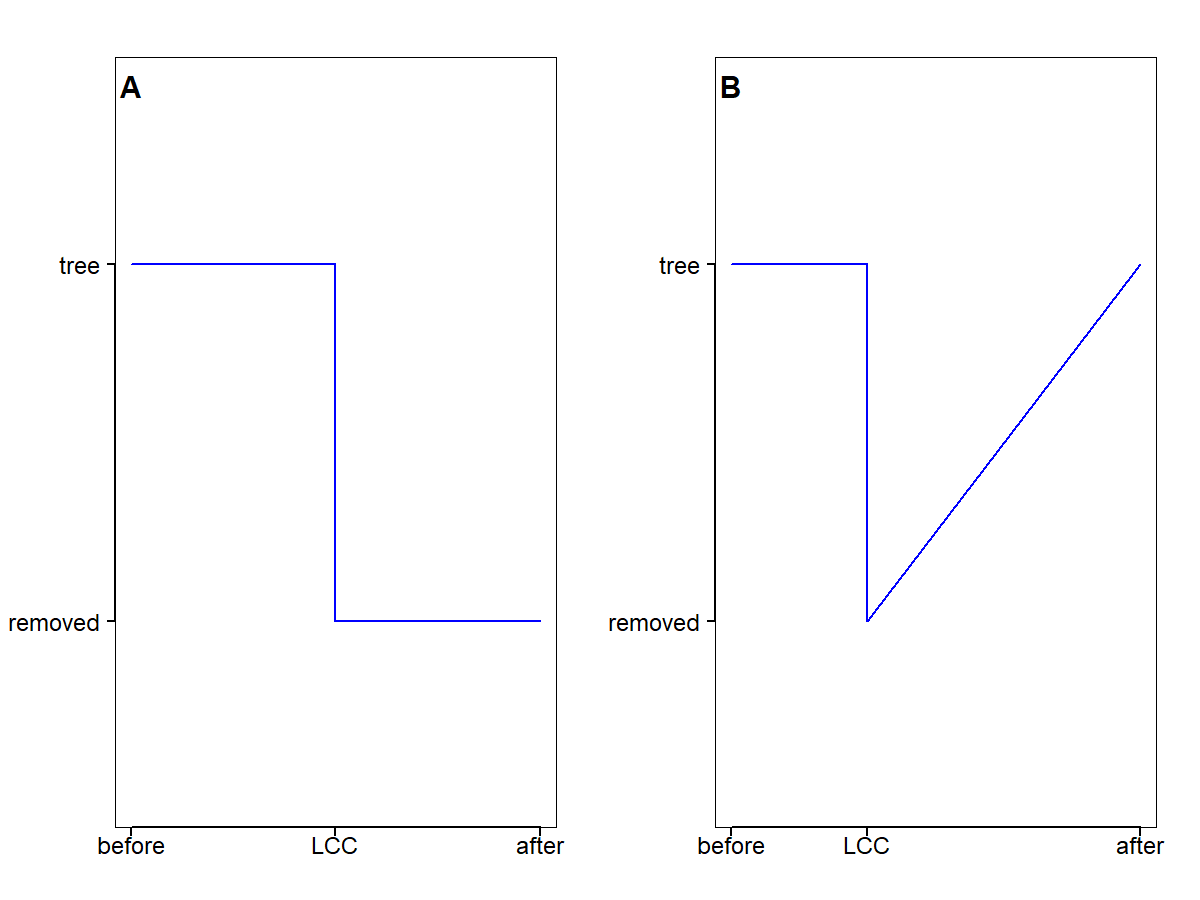
\includegraphics[width=0.7\linewidth]{figures/Fig3} \caption{The expected evolution of the land surface after trees have been removed in (A) the QLD region and (B) the NSW/VIC region.}\label{fig:figure3-tc-simple}
\end{figure}

The overall hypothesis is that the effect of 2003 - 2004 land clearings
in the QLD region and the 2003 bush fires in the NSW/VIC region cause a
step change in the local rainfall. The actual tree cover change during
this time at the pixel level was derived from the 15-year MODIS data
(discussed below). As the length of the tree cover data is shorter than
available rainfall data, earlier land clearing in the QLD region cannot
be identified spatially, hence they are excluded from the analysis.

\hypertarget{Data}{\section{Data}\label{Data}}

Several land surface data sets were used in this study. The main one was
the MOD44B product Global Vegetation Continuous Field data set (version
5). This data set provides estimates of percent tree cover (percentage
of ground surface covered by trees) at a grid resolution of 250 m
(Townshend et al., 2011), which is finer than the earlier mentioned
burned product MCD45A1. The data set is available on an annual time
interval for the study period of 2000 - 2015. The tree cover data was
produced from 16-day Terra MODIS Land Surface Reflectance data and Land
Surface Temperature (Townshend et al., 2011). The National Dynamic Land
Cover Dataset (DLCD) (Lymburner et al., 2010) from the Australian
Collaborative Land Use Mapping Program (ACLUMP) was used to verify the
trend of vegetation cover change calculated from the previous data set.
This data set, developed by Geoscience Australia and Australian Bureau
of Agricultural and Resource Economics and Sciences (ABARES), is the
first nationally consistent and thematically comprehensive land cover
reference for Australia. The DLCD is based on the 16-day Enhanced
Vegetation Index (EVI), again from the MODIS satellite, between April
2000 and April 2015. It also has a grid resolution of 250 m. The data
set provides information on the final land cover types (as in 2015) and
estimated trend of EVI statistics (annual mean, maximum and minimum).

The SILO Rainfall product data for Australia was used (Jeffrey et al.,
2001) (available online at \url{https://silo.longpaddock.qld.gov.au/}))
. The data has been projected onto a national 0.05\textdegree  by
0.05\textdegree  grid (approximately 5 km by 5 km). This gridded data
set was generated from station observations using spline interpolation
and kriging (Jeffrey et al., 2001). The data has been compared to other
gridded products and observed data and is generally of high quality
(Tozer, Kiem \& Verdon-Kidd, 2009, 2012). The data is available on a
daily and monthly basis from 1889 to current. Here a subset of 36 years
(1979 - 2015) was used. The study was conducted on monthly data, as a
land cover change effect on annual rainfall might be negligible, but can
often be significant in particular months or seasons (e.g. Otterman et
al., 1990; Gaertner et al., 2001; Semazzi \& Song, 2001; Oleson et al.,
2004; Deo et al., 2009).

Large scale climate drivers are represented by various climatic indices.
The Southern Oscillation Index (SOI) is generally regarded as a good
predictor of Australian rainfall (Risbey et al., 2009; Chowdhury \&
Beecham, 2010; Westra \& Sharma, 2010), but its skill is weaker in some
parts of Australia. For example the Southern Annular Mode (SAM) is found
to be more important than ENSO in south Western Australia (Meneghini,
Simmonds \& Smith, 2007). The testing of the suitability of each index
for the regions of interest is described in a later section. The
following climate indices were used as candidate predictors for local
rainfall.

\begin{itemize}
\tightlist
\item
  Southern Oscillation Index (SOI). The Troup version of the monthly SOI
  series used in this study was obtained from BoM (available online at
  \url{http://www.bom.gov.au/climate/current/soihtm1.shtml}).\\
\item
  Eastern, East Central and Central Tropical Pacific Sea Surface
  Temperatures (NINO 3, NINO 3.4 and NINO 4). Monthly SST anomalies are
  available from IRI/LDEO data library and the extended NINO data set is
  used (available online at
  \url{http://iridl.ldeo.columbia.edu/SOURCES/.Indices/.nino/.EXTENDED/}).\\
\item
  Pacific Decadal Oscillation (PDO). The Pacific Decadal Oscillation is
  the leading principal component of monthly SST anomaly in the North
  Pacific Ocean.. The monthly PDO series was provided by JISAO (Joint
  Institute for the Study of the Atmosphere and Ocean, University of
  Washington) (available online at
  \url{http://jisao.washington.edu/pdo/PDO.latest}).\\
\item
  Indian Ocean Dipole (IOD). The Indian Ocean dipole is commonly
  measured by the difference between SST anomaly in the western (50 -
  70\textdegree E and 10\textdegree S-10\textdegree N) and eastern (90 -
  110\textdegree E and 0 - 10\textdegree S) equatorial India Ocean (Saji
  et al., 1999). Monthly IOD was obtained from JAMSTEC (the Japan Agency
  for Marine-Earth Science and Technology) (available online at
  \url{http://www.jamstec.go.jp/frcgc/research/d1/iod/DATA/dmi.monthly.txt}).
\end{itemize}

\section{Statistical method}\label{statistical-method}

As an initial analysis a simple boxplot and t-test is used to analyse
whether there is a significant change in tree cover in time, and before
and after the suspected change in the regions.

To assess the actual causal relationship between the tree cover and the
rainfall a flexible regression model is applied (discussed in detail
below). A step change is not directly obvious in the time series of the
rainfall anomalies (Figure \ref{fig:ts-mean}) for both regions, even
though the data is deseasonalised and detrended. In this study we apply
different statistical methods to analyse the effect of tree cover change
on rainfall. Both methods make use of a regression model to remove
year-on-year variability in rainfall to strengthen the tree cover change
signal.

In the first method, the tree cover change is implemented as a factor
variable in the regression model, and the significance of this variable
is tested. In the second method, a rank sum test (step trend test), is
applied to the regression model residuals after effects of other major
factors were removed. This assumes that after removal of all climate,
long term linear trend and seasonal variation, the vegetation cover
change is the only factor explaining the non-random pattern in the
rainfall residuals.

\begin{figure}
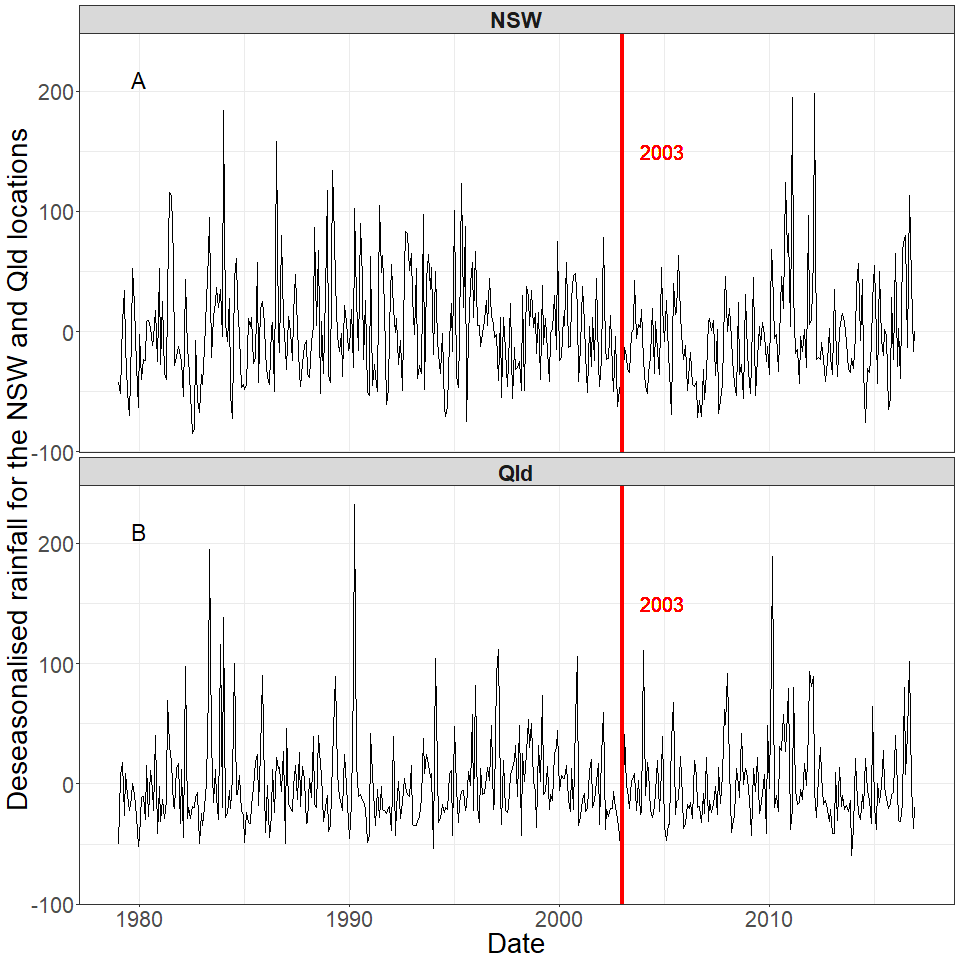
\includegraphics[width=0.9\linewidth]{figures/Fig4} \caption{The deseasonalised and detrended rainfall over the 30 years period in (a) the QLD region and (b) the NSW/VIC region. The vertical red lines indicate the year of 2003, in which the studied land cover changes occurred. A change in the time series data is not obvious before and after the land cover changes.}\label{fig:ts-mean}
\end{figure}

\subsection{Regression model}\label{reg_model}

As highlighted in the introduction, the Australian climate is influenced
by sea surface temperatures in the tropical Pacific and Indian Oceans,
as well as pressure systems in the Southern Ocean (BoM, 2012). Risbey et
al. (2009) compared five large-scale drivers, including ENSO (measured
by SOI and the Tropical Pacific Sea surface temperatures (SSTs)), IOD,
SAM, MJO (Madden-Julian oscillation) and blocking, in relation to
Australian rainfall variability. The MJO is a large scale
eastward-propagating wave-like disturbance located around equatorial
latitudes (Risbey et al., 2009). They identified SOI as the most
important index among all climate indices tested for broad parts of
Australia (including QLD and NSW/VIC) in almost any season. In this
study, four climate indices were selected from the main climatic
indicators (see section \protect\hyperlink{Data}{Data}) and used as the
explanatory variables in the model for each study region. A further
complicating factor is the influence of the ``millenium drought'' over
the study period and in particular the change to wet conditions in 2010
- 2011 (Dijk \& Viney, 2013). Therefore, the spatially averaged monthly
rainfall in the Murray Darling Basin (MDB, downloaded from
\href{http://www.bom.gov.au/web01/ncc/www/cli_chg/timeseries/rain/allmonths/mdb/latest.txt}{the
Bureau of Meteorology}) was used to explain the year-on-year variation
in the rainfall in the regions. Since both regions at least partly
overlap with the MDB, the average rainfall for the entire basin was
assumed to be a useful explaining variable.

Correlations between rainfall and each climate index were analysed.
Rainfall in each study region was first deseasonalised and detrended
using the seasonal decomposition function \texttt{ds} in the package
\texttt{deseasonalise} in R (R Core Team, 2018). Using detrended data
gives a better indication of the underlying correlation by removing the
underlying correlation in the data (Smith \& Timbal, 2012). The
cross-correlations between the deseasonalised and detrended rainfall and
the climatic indices were tested, and the strongests indicators at lag 0
were identified for the model. Because the PDO describes the
multi-decadal SST with lower frequency (MacDonald \& Case, 2005;
Zanchettin et al., 2008; Kamruzzaman, Beecham \& Metcalfe, 2011),
instead of 37-year rainfall data, a longer period (115 years, from 1900
to 2015) was used to estimate the correlation with PDO, up to lag 24.
For the other indices, the 37-year data was used.

Rainfall in Australia shows strong seasonal patterns (Holper, 2011;
Australian Bureau of Statistics, 2012). As a result a seasonal component
of rainfall has a periodic pattern which should be included in the
model. In addition, long term trends in the regional rainfall in some
parts of Australia are significant (Hughes, 2003; Gallant, Hennessy \&
Risbey, 2007; Chowdhury \& Beecham, 2010). The presence of long term
trends can be confused with the outcome of a step change in rainfall. As
a result a linear trend term was implemented in the model to remove any
long term effects.

We assumed all the factors are additive smooth components in determining
rainfall following Kamruzzaman, Beecham \& Metcalfe (2011). In this
case, the rainfall model is a generalised additive model (GAM) (Hastie
\& Tibshirani, 1986) with a log link function \texttt{g()} and assuming
the residuals are gamma distributed. We used the shrinkage version of
the cubic regression splines (Wood, 2011) as smooth function. All
splines were limited to 3 knots in flexibility (Wood, 2011), to reduce
the risk of overfitting. \vspace{0.5cm}

\begin{equation}
\begin{array}{lll}
g(E(\mathbf{R}_r)) = &\beta_0 + s_1(\mathbf{MDB_{monthlyRain}}) + s_2(\mathbf{SOI}) + s_3(\mathbf{IOD}) + \\
&s_4(\mathbf{Nino3.4}) + s_5(\mathbf{Nino4}) + s_6(\mathbf{PDO}) + \\
&s_7(\mathbf{Season}) + \beta_1\mathbf{Trend} + \boldsymbol{\epsilon}_r
\end{array}
\label{eq:model}
\end{equation}

The bold letters represent the time series vectors. The region is
indicated by \(r\), while \(\beta_u\) (\(_u\)=0, 1) are the fitted
coefficients in the model. \(s_v\) (\(_v\)=1, 2, 3,\ldots{}) are the
smooth penalized cubic regression spline functions on the climatic
indices and the season. MDB\textsubscript{monthlyRain} is the spatially
averaged monthly rainfall across the Murray Darling Basin.

The variable \textbf{Trend} = 1,2,3\ldots{}n, where n is the total
number of months in the time series is the possible long term trend in
the data, while \textbf{Season} is the seasonal component. The climatic
terms are also modelled with smooth functions as the effect of large
scale drivers on Australian rainfall can be seasonal (Murphy \& Timbal,
2008; Schepen, Wang \& Robertson, 2012).

\subsection{Tree cover change as factor variable}

One of the main difficulties in empirical observation studies related to
the effect of land cover change on rainfall is the lack of continuous
monitoring of land surface variables. Moreover, no specific variable can
possibly be defined that can clearly represent the land surface process.
Given the lack of a full picture of the land surface process, a factor
variable was used in the regression model to represent the abrupt land
surface change (see Equation \eqref{eq:model}). The change could be a
result of either land clearing or bush fires as long as it is permanent
or takes a long time to recover. As indicated we approached the problem
in two different models ways.

In the first method, the tree cover change was used as a predictor in
the regression model, represented by a factor variable \textbf{LC}. The
significance of the coefficient of \textbf{LC}, denoted as \(\beta'_5\)
in Equation \eqref{eq:model}, can be determined by a ratio test.

\begin{equation}
  \mbox{LC} = \left\{
  \begin{array}{ll}
     \mbox{Trees} \\
     \mbox{Removed}
  \end{array} \right.\\
\label{eq:dummyC}
\end{equation}

Therefore in both regions, land cover is ``trees'' for the period before
land cover change and ``removed'' for the period after the change. Here
we simply assumed that vegetation cover change has occurred on every
pixel. The remaining term \(\epsilon_r\) is the amount of rainfall that
is attributed to other unspecified factors and random errors. Hence the
regression model becomes \vspace{0.5cm}

\begin{equation}
\begin{array}{lll}
g(E(\mathbf{R}_r)) = &\beta'_0 + s'_1(\mathbf{MDB_{monthlyRain}}) + \\
  &s'_2(\mathbf{SOI}) + s'_3(\mathbf{IOD}) + \\
  &s'_4(\mathbf{Nino3.4}) + s'_5(\mathbf{Nino4}) + s'_6\mathbf{PDO} + s'_7\mathbf{Season} + \\
  &\beta'_1\mathbf{Trend} + \beta'_2\mathbf{LC} + \boldsymbol{\epsilon'}_r
\end{array}
\label{eq:model2}
\end{equation}

One of the difficulties is to point an exact time to the changes in the
vegetation cover in the two regions. In the QLD region, no exact time
can be assigned to the land clearing. According to the SLATS reports,
the most substantial clearing occurred between 2003 - 2004 . However,
the information on the change in type of land cover during the time
period is missing. Therefore, four scenarios were initially tested in
the analysis, however there was no real difference between these
scenarios. In the NSW/VIC region, severe bush fires were reported in
early January 2003. Hence the ``tree'' cover state was up to December
2002 then it was changed to ``removed'' state from January 2003. As a
starting date, the regression model was run from 1979 for both regions.

\subsection{Step trend test}\label{step-trend-test}

To support the regression analysis, a Mann-Whitney Rank-Sum step trend
test was used to detect changes in rainfall as a result of vegetation
cover change. This specific nonparametric statistical test was modified
from the Mann-Whitney U test by Hirsch \& Gilroy (1985) and can identify
a step change in data which is cross-correlated. In this case, this is
important as the gridded rainfall dataset has a high spatial correlation
between neighbouring pixels. The advantages of using the Rank-Sum test
are: (1) it does not depend on assumptions of the data distribution; (2)
it is not restricted to datasets with no missing data; (3) it is robust
and not as easily influenced by outliers and negative numbers (Hirsch \&
Gilroy, 1985). However, the test has less power than parametric tests.
As a nonparametric rank-based test, it depends on the ranks of the data.

The rainfall residuals from the regression model in Equation
\eqref{eq:model2} were used. The assumption is that the regression model
deseasonalises and detrends the rainfall data (Hirsch \& Gilroy, 1985),
amplifying the local landuse effects. For each month, rainfall residuals
of each year were ranked in an ascending order. The ranking of January
rainfall in a sample pixel k in QLD is illustrated in Table
\ref{tab:exampleRank}.

\begin{table}[t]

\caption{\label{tab:exampleRank}Example of ranking rainfall residuals}
\centering
\begin{tabular}{rrr}
\toprule
Year & Rainfall residuals & Rank $R'_{1k}$\\
\midrule
1998 & -0.3 & 6\\
1999 & -60.9 & 2\\
2000 & -16.1 & 4\\
2001 & -71.7 & 1\\
2002 & 111.1 & 7\\
\addlinespace
2005 & -7.2 & 5\\
2006 & -60.5 & 3\\
\bottomrule
\end{tabular}
\end{table}

The before and after period in the data formed two groups of samples.
The split point of the two periods was based on the timing of the
vegetation cover changes. In the QLD region, changes occurred anytime
during 2003 and 2004. In contrast to the previous method, the time
period covering the land cover change was excluded, as the nonparametric
test allows missing data and the power of the test is greater if data of
the change period is ignored (Hirsch \& Gilroy, 1985). As a result, the
post change period was 2005 - 2015 for the Queensland location.

In the case of NSW/VIC, the bushfires broke out in early January 2003.
The change was within a relatively short period of the year. Therefore
the post change period in this region still started in January 2003. The
pre change period was set to five years (1998 - 2002) in both regions.

The rank of rainfall in month j year i in pixel k is denoted as
\(R'_{ijk}\). The sum of ranks of rainfall in month j in pixel k before
the known intervention is:

\begin{equation}
  W_{jk} = \sum_{i=1}^{n_1}R'_{ijk}.
  \label{eq:Wj}
\end{equation}

\(n_1\) is the number of years before the land cover change. The
expected value of \(W_{jk}\) is

\begin{equation}
  \mu_w=n_1(n_1+n_2+1)/2
\end{equation}

\(n_2\) is the number of years after the change. Hence the expected
value of the rank sum before the intervention is the same for all months
and all pixels. The sum of ranks for the whole time period is fixed, as
\((n_1+n_2)(n_1+n_2+1)/2\). In this study, since there are only two
groups (before and after), knowing the rank-sum of one group is the same
as knowing the rank-sum of the other group. If the rainfall data is
temporally and spatially independent, the variance of \(W_{jk}\) is

\begin{equation}
  \sigma^2_w = n_1\cdot n_2(n_1+n_2+1)/m
\end{equation}

where m is the number of months which is 12 in the case of a full year.

Here the deseasonalised and detrended data shows little autocorrelation
in time, but possesses strong cross correlation between neighbouring
pixels, i.e. \(R>0.99\).

The sum of \(W_{jk}\) for a block of \(ns\) pixels over the whole year,
\(\sum_{j=1}^{12}\sum_{k=1}^{ns}W_{jk}\), has mean

\begin{equation}
  E(\sum_{j=1}^{12}\sum_{k=1}^{ns}W_{jk})=12\cdot ns\cdot\mu_W
\end{equation}

and variance

\begin{equation}
  Var(\sum_{j=1}^{12}\sum_{k=1}^{ns}W_{jk})=\sum_{j=1}^{12}\sum_{k=1}^{ns}\sum_{h=1}^{ns}C(W_{jk},W_{jh}).
\end{equation}

\(C(W_{jk},W_{jh})\) is the covariance of the W statistics between pixel
k and pixel h in month j. When \(k=h\), \(C(W_{jk},W_{jh})=\sigma^2_w\).
When \(k\neq h\),

\begin{equation}
  C(W_{jk},W_{jh})=\sigma^2_w r(R_k,R_h)
\end{equation}

where \(r(R_k,R_h)\) is the product moment correlation coefficient of
the concurrent ranks in pixel k and h. Here \(r\) is calculated on the
full time series in each pixel. In the analysis, the test was applied to
a square block of four pixels each time. As argued by Hirsch \& Gilroy
(1985), \(ns=4\) is the most optimal solution to balance the cost and
the gain in the test power.

The statistic of the step trend test is then defined as

\begin{equation}
  Z'=\frac{\sum_{j=1}^{12}\sum_{k=1}^{ns}W_{jk}-12\cdot ns\cdot\mu_w}{\sqrt{Var(\sum_{j=1}^{12}\sum_{k=1}^{ns}W_{jk})}}.
  \label{eq:Z}
\end{equation}

The above statistic is written for a 12 month period. By changing the
value 12, it can also be used to test seasonal rainfall change or for
other customized periods.

\begin{table}[t]

\caption{\label{tab:Zscore}The interpretation of Z' score in the step trend test}
\centering
\begin{tabular}{l}
\toprule
 \\
\midrule
$Z'>0$  and rainfall decreases after change\\
$Z'<0$ and rainfall increases post change\\
$Z'=0$ and rainfall does not change\\
\bottomrule
\end{tabular}
\end{table}

The null hypothesis (\(H_0\)) in this study is that there was no change
in rainfall due to land surface intervention. The results of the step
trend test can be interpreted according to the sign of the Z' score (see
Table \ref{tab:Zscore}, Chapter 23, P887 (Hipel \& McLeod, 1994)), and
is normally distributed similar to the standard normal statistics Z.

As part of the analysis, the ``field significance'' of the Z' score test
was considered to improve the interpretion of the step change at
regional scales from multiple local tests (Wilks, 2006; Westra,
Alexander \& Zwiers, 2013). Here, the bootstrapping resampling method
from Westra, Alexander \& Zwiers (2013) was used to evaluate the field
significance. This means the spatial structure of the pixels was
maintained, but the order of the years and months was changed by random
resampling. For each resampling, the test statistic identifies the
percentage of the pixels with a significant positive or negative step
change for the step trend test. The test statistics on 1000 resampled
replicates were used to develop the distribution of these percentage
values.

\section{Results}\label{results}

\subsection{Tree cover change}\label{tree-cover-change}

The pixels, where the tree cover change based on the MOD44B data was
significant (\(p \leq 0.05\)) in each study region, are shown in Figure
\ref{fig:tctrend} for the NSW/VIC region (A) and the QLD region (B). In
the QLD region there actually has generally been an increase in tree
cover after the clearing of native vegetation stopped. In the NSW/VIC
region, much of the tree loss between 2002 and 2003 was concentrated in
the Snowy Mountains close to the border of NSW and VIC, which is also
evident in the figure. Tree cover loss occurred in large parts of the
QLD region between 2002 and 2005, but this tree loss was spatially less
concentrated.

\begin{figure}
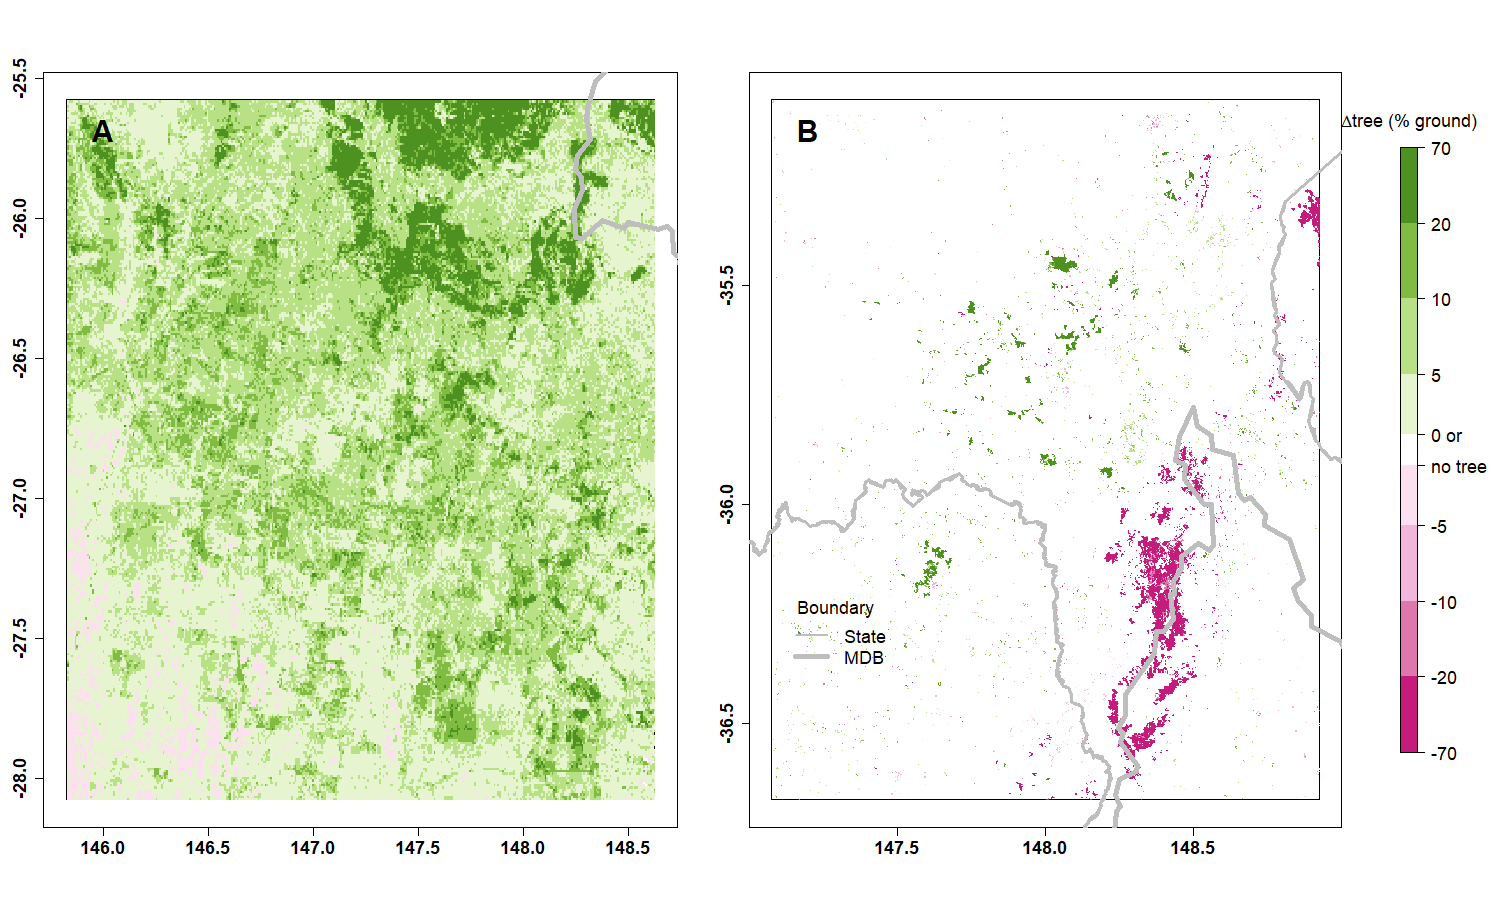
\includegraphics[width=0.9\linewidth]{figures/Fig5} \caption{The maps show significant changes in tree cover identified from the MOD44B data between 2003 and 2015 in the Qld region (A) and the NSW/VIC region (B). The amount of change was calculated as the difference in tree cover before and after the specified land cover intervention and it is shown as the percentage of the ground area. Green colour indicates an increase in tree cover, while red colour indicates a decrease in tree cover.}\label{fig:tctrend}
\end{figure}

\subsection{Regression Model}\label{regression-model}

The correlation between the climatic indices and rainfall in the regions
(See the supplementary material with this paper) indicated that for both
regions the PDO had the weakest correlations, and this factor was
therefore dropped as a predictor. Although some indices are serially
correlated with rainfall up to several months, the lag zero events have
the greatest correlation coefficients. Furthermore, using multiple
climatic index series was generally found most useful in rainfall
prediction (e.g. Risbey et al., 2009; Kamruzzaman, Beecham \& Metcalfe,
2011).

\begin{figure}
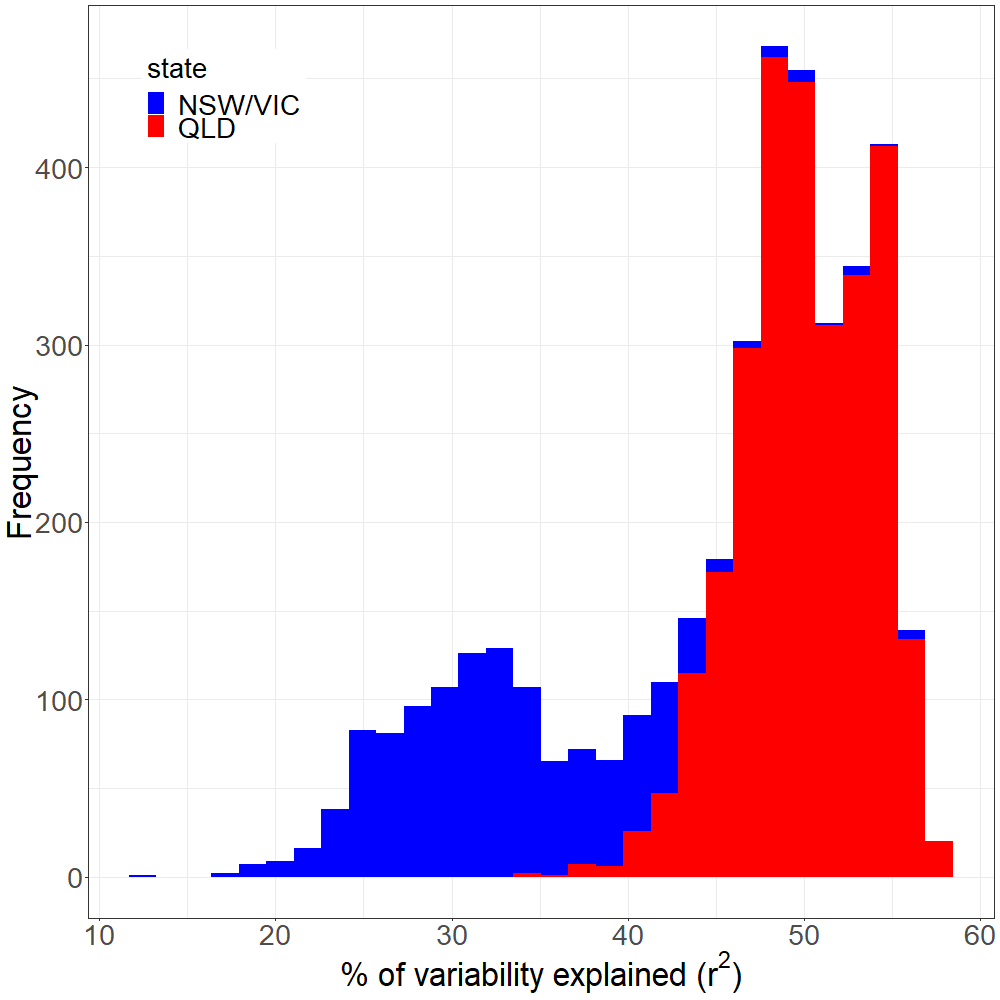
\includegraphics[width=0.7\linewidth]{figures/Fig6} \caption{The distribution of the variance explained (adjusted $r^2$ ) by the full regression model}\label{fig:rsqmodel}
\end{figure}

Generally the regression model only explains a limited amount of the
rainfall variability (Figure \ref{fig:rsqmodel}). The model in Equation
\eqref{eq:model2} accounts for an average around 33\% of the variation in
the NSW/VIC region and about 50\% of the variation in the QLD region as
indicated by the adjusted \(r^2\). The adjusted \(r^2\) is the
coefficient of determination, a measurement of the amount of variability
predicted by the model adjusting for the number of explanatory terms.

In terms of predictors of the local rainfall in the model, logically,
the average rainfall across the larger Murray Darling Basin is highly
significant. This confirms that this variable is a good reflection of
the year on year variability in the rainfall. The model also confirms
the importance of the climate drivers and the seasonality in Australian
rainfall, as many of these variables were significant. Even at the grid
level, the seasons and several of the climatic indices were significant
(\(p \leq 0.05\)) everywhere in both regions. The climate drivers (at
lag zero) accounted, on average, for 6.5\% of the rainfall variability
in both the QLD region and the NSW/VIC region (see Figure \ref{fig:rsq}
for the distribution of adjusted \(r^2\) in these two regions). These
figures are within the upper bound of seasonal rainfall predictability
by a SST anomaly field reported by Westra \& Sharma (2010).

\begin{figure}
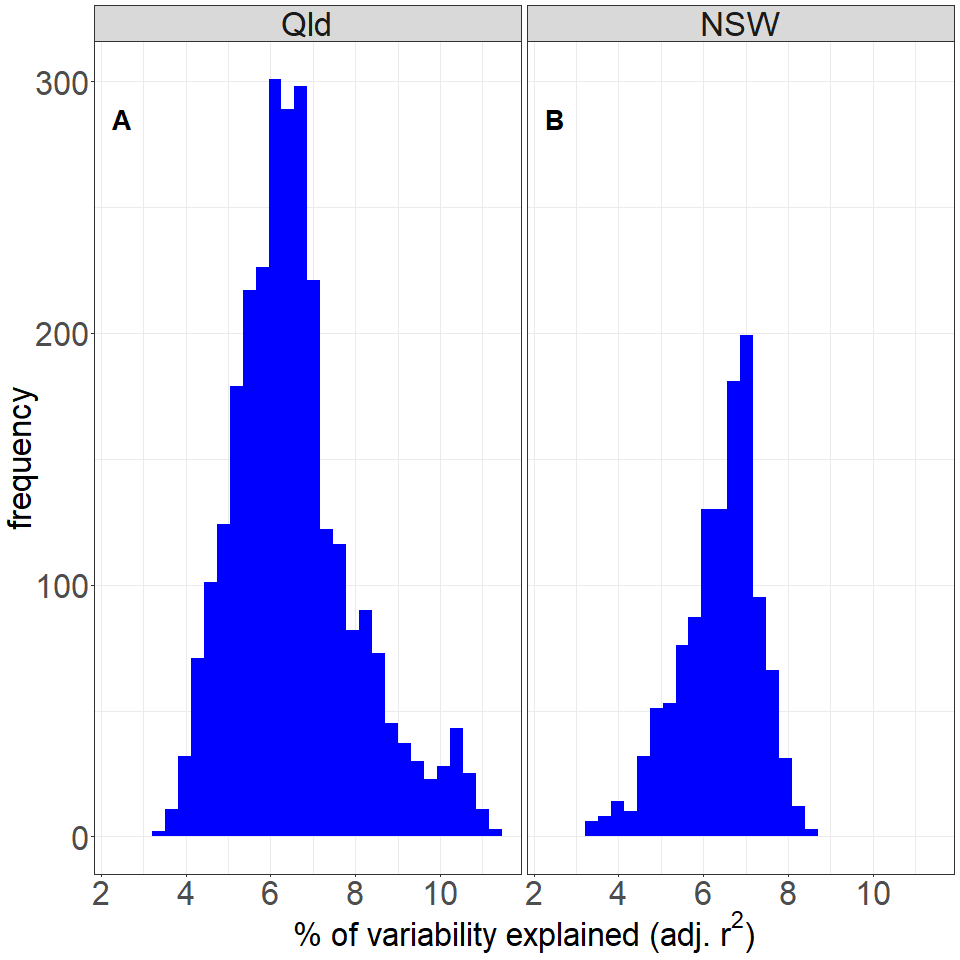
\includegraphics[width=0.7\linewidth]{figures/Fig7} \caption{The performance of the regression model if rainfall is only modelled by the climate drivers. It shows the percentage of rainfall variability that can be explained by the climate drivers for the Qld (A) and NSW/VIC (B) region}\label{fig:rsq}
\end{figure}

There were generally no statistically significant long term trends in
both regions. However, the trend term was kept in the regression model
to ensure the detection of step change was not due to a possible long
term trend (even if this was not significant).

\begin{figure}
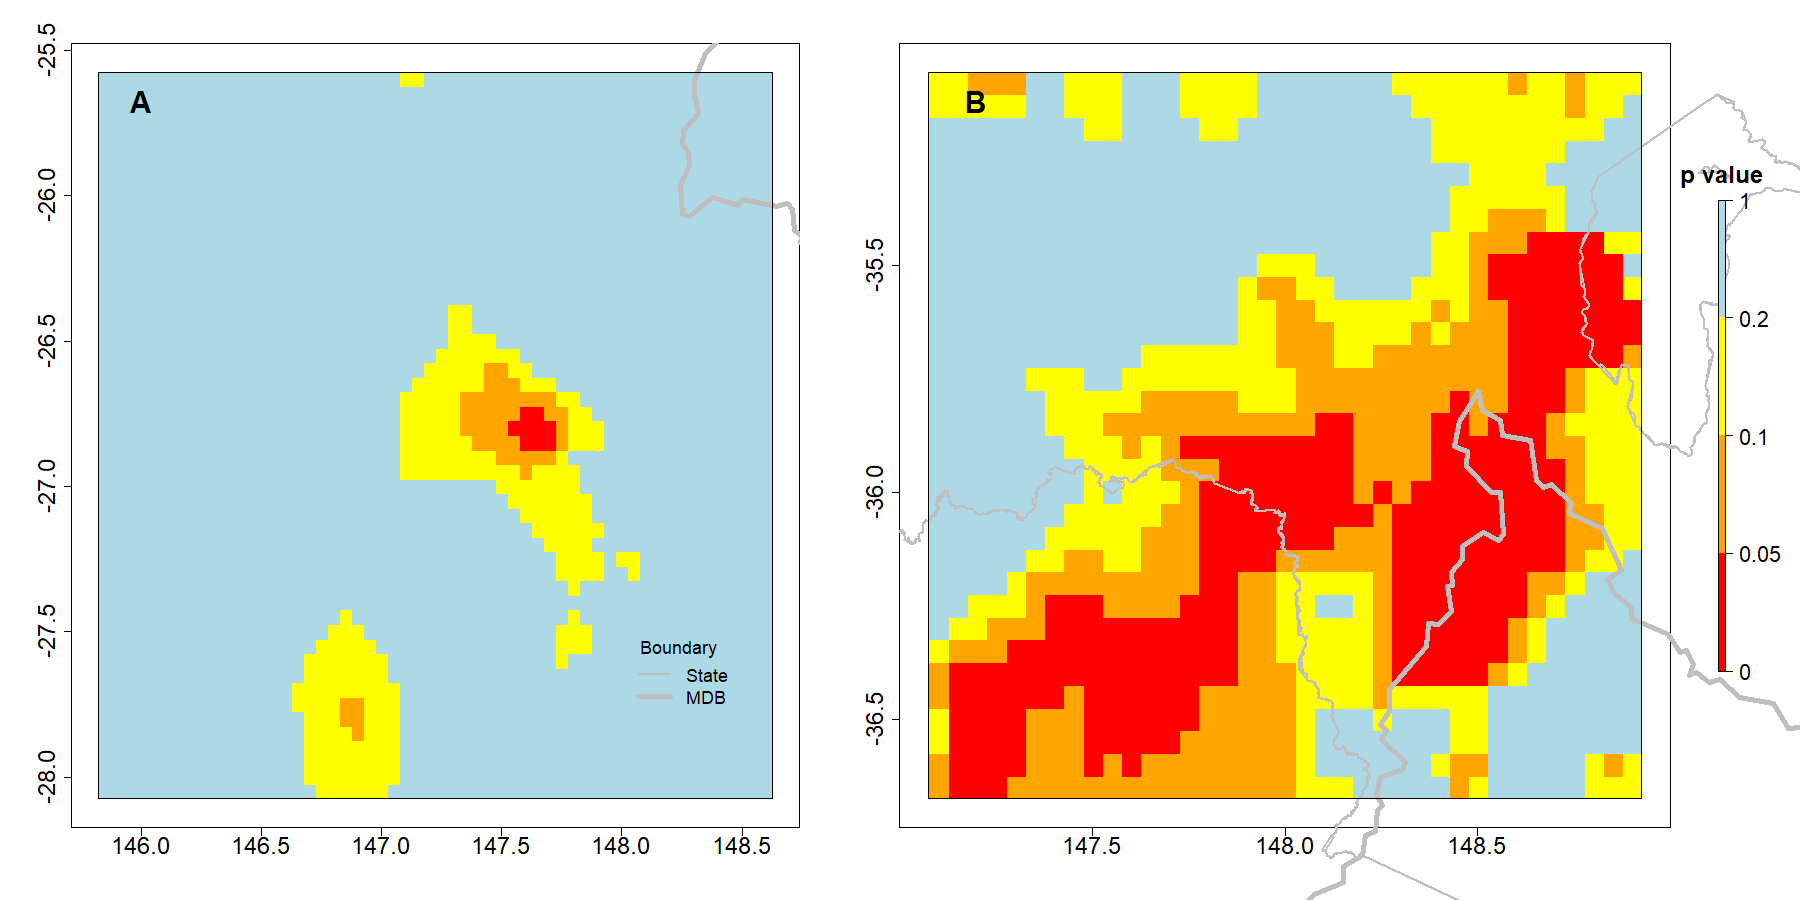
\includegraphics[width=0.9\linewidth]{figures/Fig8} \caption{The spatial distribution of significance of land cover step change variable in the GAM model predicting changes in rainfall in the both regions, the Qld region (A) and the NSW/VIC region (B). The outlines of relevant Australian states and the Murray Darling Basin are indicated in grey. The p-value reported is for the land cover variable in the model.}\label{fig:LCp}
\end{figure}

The land cover variable in the model (Equation \eqref{eq:model2}) aims to
identify a step change in the rainfall before and after the observed
change in land cover. The variable was mainly significant
(\(p \leq 0.05\)) for the rainfall estimates in some areas in NSW/VIC,
as shown in Figure \ref{fig:LCp} (B). However, the number of pixels
where the landcover variable was significant was much greater in NSW/VIC
compared to the number in the QLD region (Figure \ref{fig:LCp} (A)).
There was also some relationship between the areas of bushfires in
Figure \ref{fig:bushfire}. Only a very small area with a significant
step change due to the land cover changes was found in rainfall in the
QLD region (A)

More generally, the model for NSW/VIC suggests that the land cover
variable has a positive impact on rainfall in both regions. The fitted
coefficients for the Land cover change variable were consistently
positive for the ``tree'' part of the series. It implies that rainfall
was higher when the surface was covered by trees.

\subsection{Stronger step trend in NSW/VIC compared to
QLD}\label{stronger-step-trend-in-nswvic-compared-to-qld}

\begin{figure}
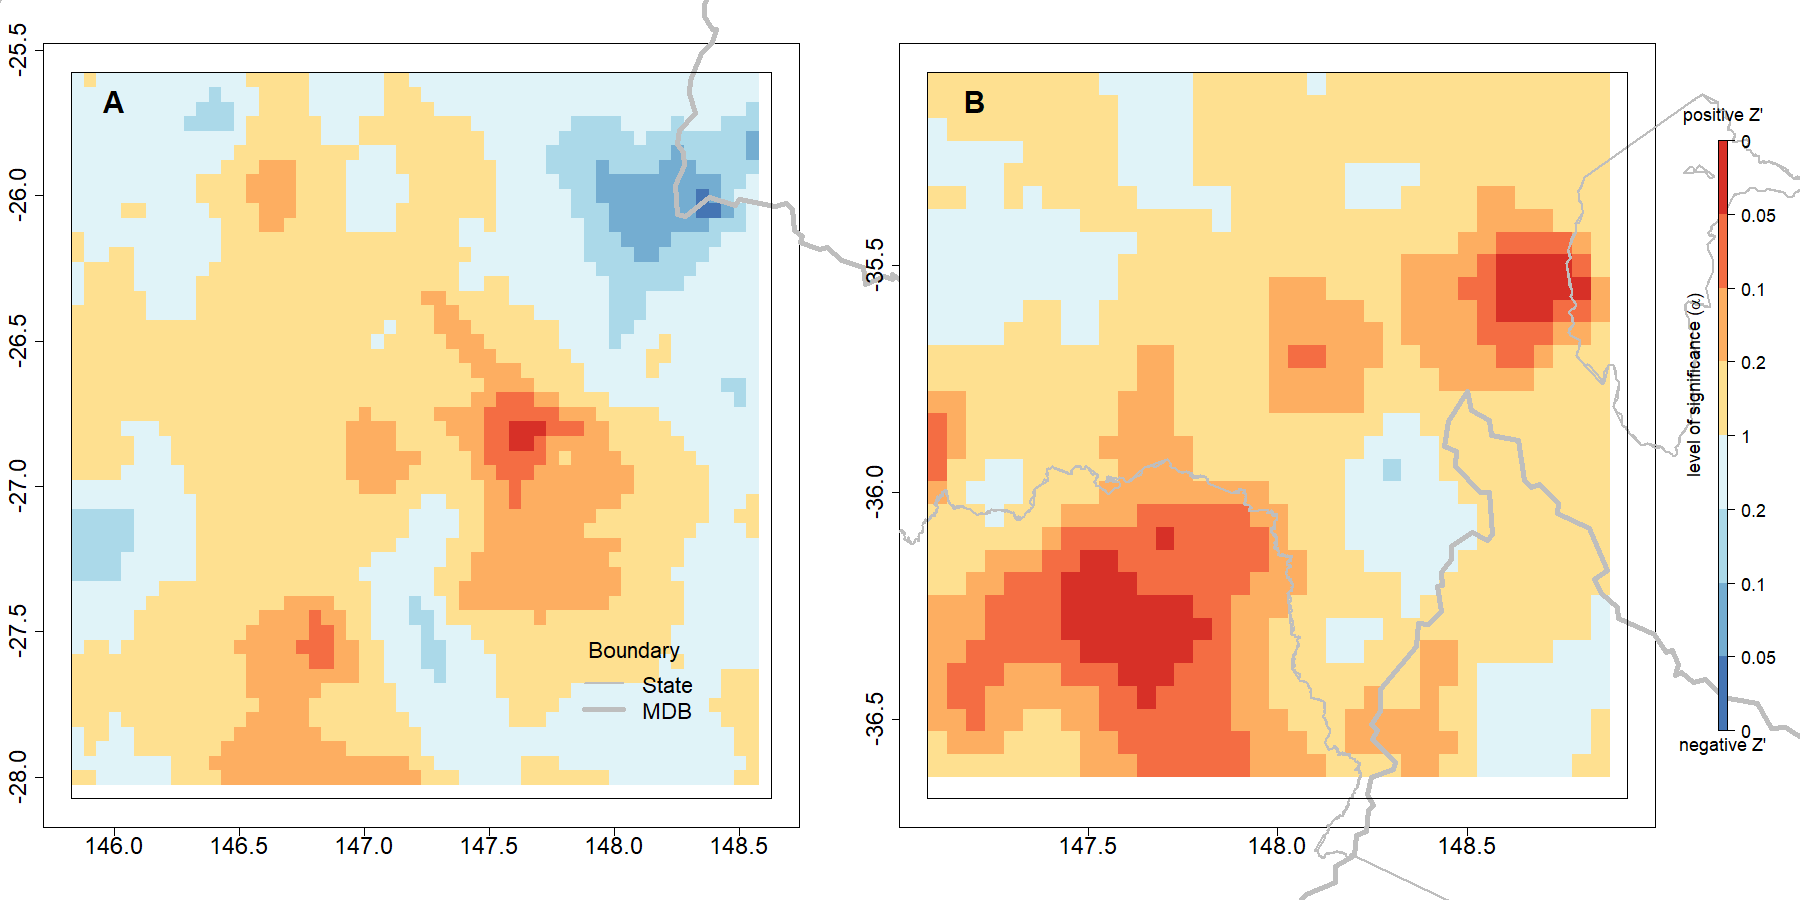
\includegraphics[width=0.9\linewidth]{figures/Fig9} \caption{Spatial distribution of the step trend test Z' statistics in the two study sites, the QLD region (A) and the NSW/VIC region (B). Warm colours (yellow, orange and red) are for positive Z' values which indicate decreasing rainfall trend due to the land surface change. Cold colours (light blue to blue) are for negative Z' values which indicate increasing rainfall trend. The deeper the colour, the more significant the statistic.}\label{fig:steptest30}
\end{figure}

In both regions there are areas of positive Z' values which imply a
decrease in rainfall (Figure \ref{fig:steptest30}), but this is stronger
in the NSW/VIC area (B) than in the QLD area (A). Qualitatively the
locations where changes in tree cover occurred in the NSW/VIC area
(Figure \ref{fig:tctrend} (B)) seem to agree with the patterns in the Z'
scores. However, a direct relationship would not necesssarily be
expected as movement of air masses could mean that actual changes of
rainfall are observed close by, but not necessarily exactly at areas
with changes of landcover. For the QLD region (A) there are only a few
significant Z' scores which matches the earlier significance in the
landcover variable in the full regresion. In the QLD region, only 0.2\%
of the pixels obtained a positive Z' score with p \(<\) 0.1. In the
NSW/VIC region (B) 3.7\% of pixels have a positive Z' score with p \(<\)
0.1. In general it is only a small proportion of both study regions.

\begin{figure}
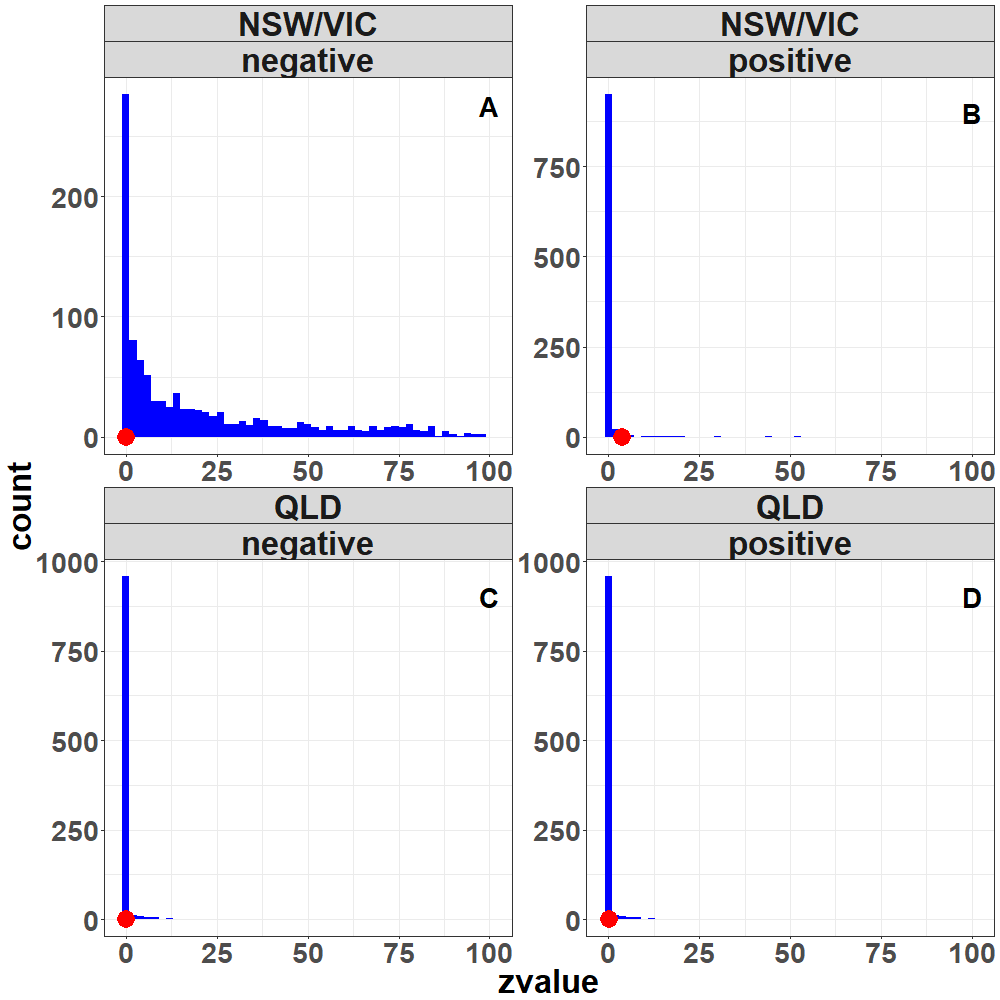
\includegraphics[width=0.7\linewidth]{figures/Fig10} \caption{Field significance results showing the distribution of percentage of significant Z' scores for the resampled series (blue bars), and the precentage significant Z' scores for the original series of rainfall years (red circle)}\label{fig:fieldsig}
\end{figure}

The rainfall regression residuals without the landcover variable for the
two regions (before-change since 1979 and after-change) were also
compared using a simple t-test. The mean rainfall residuals were
significantly different (\(p < 0.05\)) between the ``before'' and
``after'' periods in both regions. For the Queensland locations, the
mean monthly rainfall residuals were slightly lower (\(p < 0.05\)) after
the change in landcover (\(~ 0.45 mm/month\)). For the NSW/VIC locations
there was larger decrease in the mean monthly rainfall residual
(\(p < 0.05\)) post change (\(~ 1.5 mm/month\)).

The observed fraction of significant Z' scores (at \(p < 0.1\)) is
plotted on the results of the bootstrap distribution (Figure
\ref{fig:fieldsig}). The results support the earlier Z' score results.
Only the percentage significant positive Z' scores, indicating a
decrease in rainfall for the NSW/VIC region as a result in a decrease in
tree cover, falls on the tail of the field significance distribution,
while all the others are well within the distribution. This suggests
that the percentage of significant positive Z' scores in the NSW/VIC
region is least likely due to a unique series of rainfall years, but is
most likely due to changes in landcover. In other words, in the NSW/VIC
region it is most likely that the change in landcover (decrease in tree
cover) caused a decrease in the rainfall.

\section{Discussion}\label{discussion}

\begin{table}[t]

\caption{\label{tab:summarytable}Summary table of all tests on the two regions }
\centering
\resizebox{\linewidth}{!}{
\begin{tabular}{lll}
\toprule
Test & Qld & NSW VIC\\
\midrule
LC variable & Small area of significant pixels in the centre & Large area possibly aligning with bushfire affected area.\\
t-test regression model residuals & Slightly lower mean residual ($p<0.05$) after change (0.5 mm per month) & Lower mean residual ($p<0.05$) after change (1.5 mm per month)\\
Positive score & 0.2\% of pixels at $p<0.1$ & 3.7\% of pixel at $p<0.1$\\
Field significance \% of scores & Both positive and negative \% within random distribution & Positive \% outside random distribution.\\
\bottomrule
\end{tabular}}
\end{table}

Overall the summary table (Table \ref{tab:summarytable}) of the results
indicates that the effects of land clearing or bushfire on rainfall are
consistent across the range of different statistical tests. In all
cases, the data for the NSW/VIC region indicates statistical evidence
that the reduction in tree cover (the land cover change) resulted in a
local decrease in rainfall. In contrast, the data for the QLD region
indicates lower statistical evidence that the loss of trees due to land
clearing resulted in reduction in the rainfall (Table
\ref{tab:summarytable}).

Generally, empirical studies on LCC-precipitation interaction are
conducted within an area with known land surface intervention (e.g.
Otterman et al., 1990; Durieux, Machado \& Laurent, 2003; Negri et al.,
2004; Sato, Kimura \& Hasegawa, 2007). However, these locations are rare
and difficult to isolate from real landscape change. Modelling studies
are abundant (e.g. Chagnon \& Bras, 2005; Wang et al., 2009; Pinto et
al., 2009), but these are generally not directly linked to observed
data. In this study we tested the effect of land cover change across a
broad region, which included locations where changes were known to occur
or have occured. The advantage of the current approach is that long time
series of land cover data are not required. Furthermore, it does not
assume a specific relationship between vegetation cover change and
rainfall but allows the data to show this relationship, by applying the
analysis to a broader area outside the boundary of the vegetation cover
change. This approach is expected to provide a way to reduce the risk of
a false positive paradox, by comparing results between areas with and
without vegetation cover change.

Overall the results suggest that at least for the NSW/VIC region, a
decrease in tree cover causes a decrease in rainfall. However, there are
several possible complicating factors in the data that require
discussion.

\subsection{Rainfall variability}\label{rainfall-variability}

Rainfall in Australia is highly variable from year to year, and the time
period in this study included a severe drought (Dijk \& Viney, 2013), as
well as the drought breaking years 2010 and 2011. The purpose of using
the regression model is to remove the year to year and month to month
variability in rainfall and therefore strengthen the land cover signal
in the residuals. We used the spatially averaged monthly rainfall
timeseries for the larger Murray Darling Basin (Figure \ref{fig:selreg})
to remove the general variability. However, overall the model does not
explain more than 50\% (QLD) and 30\% (NSW/VIC) of the rainfall
variability (Figure \ref{fig:rsqmodel}), and only around 7\% on average
is due to the climate drivers (Figure \ref{fig:rsq}). And while this is
consistent with the literature e.g. Westra \& Sharma (2010), this means
some variation due to external factors could still be left in the
residuals. Rainfall is generally considered a stochastic process (e.g.
Fowler et al., 2005; Cowpertwait, Salinger \& Mullen, 2009; Burton et
al., 2010) and some of the variability could either be a different
response to a combination of climate factors (as interactions were not
tested in the model), or a non-stationary response to the climate
drivers. The severe bushfires in 2003 were also triggered by the extreme
drought conditions during the millenium drought (Dijk \& Viney, 2013).
Although the effect of the drought on the overall rainfall quantities
has been accounted for in part by the model, a further delayed or
cumulative effect of the drought could be feeding into the local
land-atmosphere interaction. As a result, the rainfall feedback to the
vegetation cover change could be weak under the dry conditions between
2001 and 2009, and this could have affected the result.

The fact that no significant long trend was identified, may not disprove
a long term trend in rainfall, as overall time period is fairly short
(Koutsoyiannis, 2006). Removing the long term trend could mean more
pixels in NSW/VIC would indicate a significant step change.

\subsection{Vegetation dynamics}\label{vegetation-dynamics}

The second possible effect is the dynamic nature of the vegetation
clearing and recovery, especially for the QLD region. Not only does this
refer to a change in the total biomass, but this could also include a
change in the species composition as a result of the disturbance.

Although land clearing has occurred at a high rate and broad scale in
Queensland (Department of Science, Information Technology and
Innovation, 2017), the clearing does not have a clear start and end
point. QLD has a long history of land clearing. According to the series
of SLATS reports on land cover changes in QLD released by the Queensland
government, land clearing continued in and around the study region
between 1988 - 2008. Major broad scale and high rate clearings occurred
in 1999 - 2000 and 2002 - 2004 (Figure \ref{fig:slat}). And even though
there was a decrease in land clearing post 2005, it is difficult to
define a clear cut change in the tree cover in this region.

The specific vegetation class in the Queensland area is also well-known
for rapid regrowth and ``thickening'' in favourable conditions (Gowen \&
Bray, 2016), and this could explain the increase in vegetation cover in
2015 in the Qld area (Figure \ref{fig:tctrend}). This again, could also
be related to a change in the vegetation composition further
complicating the analysis. In particular the favourable rainfall years
of 2010 and 2011 would have boosted regrowth, increasing
evapotranspiration and therefore decreasing the effect of the rainfall
change.

\begin{figure}
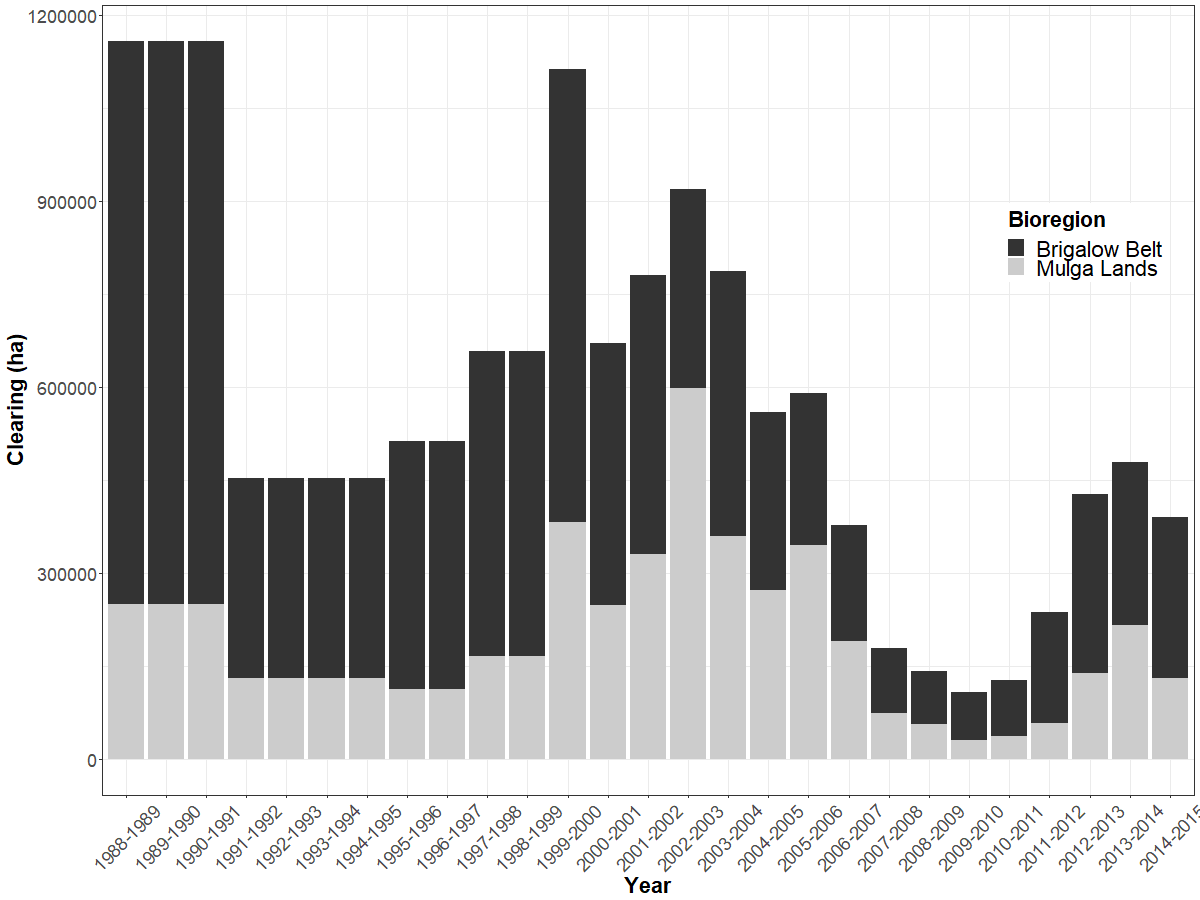
\includegraphics[width=0.9\linewidth]{figures/Fig11} \caption{Woody vegetation clearing rate in QLD for the two major bioregions in the study area. The data were obtained from SLATS (2017), and clearly indicate a sharp decrease in the clearing rate after 2005.}\label{fig:slat}
\end{figure}

The different causes of vegetation cover change in these two regions
could lead to different post-change characteristics. The trends in EVI
in the QLD region are opposite to the NSW/VIC region, based on the DLCD
data. This could also be due to the lower tree density in the QLD region
compared to the NSW/VIC region before land surface interventions. In
contrast, the significant bushfires (Figure \ref{fig:bushfire}) would
have drastically reduced the vegetation cover and recovery was very slow
in some areas within the NSW/VIC area. The persistent drought in the
2000s (Howden, 2012; Dijk \& Viney, 2013) delayed the regrowth of trees.
Conversely, replacing tree cover with pasture and crops in the Qld area
might only have a relatively subtle impact on the EVI.

\subsection{Gridded monthly rainfall
data}\label{gridded-monthly-rainfall-data}

The rainfall data used in this study is gridded. This data set is robust
and consistent over a long time series (from 1900 to current) and has a
broad national wide coverage which can provide more information
spatially (Jeffrey et al., 2001; Tozer, Kiem \& Verdon-Kidd, 2009).
However, high cross correlation between pixels, due to the interpolation
method in this data set (Jeffrey et al., 2001), can also introduce
spatial noise. In the step trend test the cross correlation was
accounted for. However, some other methods are also available, which
could be used to perform a comparative trial. For example, Narisma et
al. (2007) applied a spatial Gaussian filter on a similar data set and
used wavelet analysis to detect a step change in rainfall. High quality
station data is another option to test whether the observed spatial
pattern in the step trend test results was not due to the gridded data
itself. Resampling methods, such as bootstrapping and permutation (used
in this study) (Wilks, 1997; Kundzewicz \& Robson, 2004; Westra,
Alexander \& Zwiers, 2013), can also be used to further assess the
strength of the significance of results . While the gridded data set is
most useful in regions with sparse rain gauge networks, such as in this
study, it can actually reduce information where the rain gauge density
is high (Jones, Wang \& Fawcett, 2009). In the NSW/VIC region, the
coverage of rainfall stations is more intensive, but they are mainly
located in the valleys. As a result, the interpolated data might be a
limited representation of the true local rainfall.

\subsection{General approach}\label{general-approach}

Parametric tests are generally more powerful than nonparametric test in
detecting a trend, when the data is normally distributed (Onoz \&
Bayazit, 2003; Kundzewicz \& Robson, 2004). As a non-parametric test,
the step trend test has the advantage of being distribution free and
having no restriction on missing data (Hirsch \& Gilroy, 1985). On the
other hand, the disadvantages of non-parametric tests, such as being
limited to hypothesis testing and being weaker in power, also hold for
the step trend test (Whitley \& Ball, 2002).

Overall, the current study provides a statistical data based approach,
building on several lines of evidence to reject the null hypothesis (no
step change in rainfall occurs as a result of tree cover loss) at least
for the NSW/VIC region. Limited by the available data, the time frame
under study had to include a long lasting drought period (Holper, 2011;
Dijk \& Viney, 2013). The strong impact of this prolonged drought might
have suppressed the land-atmosphere interaction and modified the cause
and effect relationship between rainfall and vegetation cover change.
This could be one of the reasons that the land cover change effects on
the local climate found in other studies (e.g. Görgen et al., 2006;
McAlpine et al., 2007) do not appear in the QLD region.

Future research will include additional areas to further test the
approach in this study. However, such areas are not easy to find. There
are several requirements for a good study area:

\begin{enumerate}
\def\labelenumi{\arabic{enumi}.}
\tightlist
\item
  It needs to be large enough to capture the effect of landuse on
  rainfall within the area;\\
\item
  It needs to have a drastic enough landuse change to be observable
  above the rainfall variation;\\
\item
  It needs to have a long enough climate data time series both prior and
  post landuse change.
\end{enumerate}

The obvious locations have always been Amazonia and sub-Saharan Africa,
where also most of the modelling studies have taken place (Kucharski,
Zeng \& Kalnay, 2013; Pitman \& Lorenz, 2016). The problem with the
sub-Saharan location is that the land use change is quite long ago and
local data is difficult to obtain. The problem with the Amazonian
location is that this area is well-known for the feedback and we felt
that we could not add much to this work. We propose that it would better
to focus on areas affected by bushfires, as we did with the NSW/VIC
location. The recent bushfires in California and Colorado could
potentially be good locations, but at the moment there is insufficient
``post event data''. Further work could also focus on identifying an
area that has been impacted by land cover change, but does not include a
significant drought period.

While the power of the test can be improved with the longer length of
the post-intervention period (Hirsch \& Gilroy, 1985), the dynamic
nature of vegetation regrowth in this case study also affects this
effect. A better approach might be to build a global study that
investigates multiple locations where drastic landcover changes have
taken place, which would also remove some of the climate variability
effects due to the larger sample size.

\section{Conclusions}\label{conclusions}

In this study, we present a statistical approach to identify the impact
of a change in land cover on local rainfall.The results, based on
gridded rainfall data found, that a reduction in vegetation cover is
likely to have reduced local rainfall for a large area in NSW/VIC
affected by bushfires. However, land clearing in QLD was unlikely to
have reduced rainfall over the same time period.

Drought may have had a pronounced impact on the land surface condition
during the study period, such asleading to significant reduction in
vegetation cover and extreme events such as bushfires. The lack of
rainfall and associated high temperatures may mask the impact on
rainfall of a step change in the vegetation cover. Hence, the signal of
Land Cover Change feedback on rainfall is probably weaker under such
regional dry conditions, as the impact of Land Cover Change on rainfall
is mainly through changes in moisture convergence (Görgen et al., 2006;
Pitman \& Hesse, 2007).

\section*{References}\label{references}
\addcontentsline{toc}{section}{References}

\hypertarget{refs}{}
\hypertarget{ref-ABARES2010}{}
ABARES. 2010. Land use of Australia, Version 4, 2005/2006.

\hypertarget{ref-ABC2003}{}
ABC News. 2003. Kosciuszko slow to recover from bushfires.

\hypertarget{ref-ABS2012}{}
Australian Bureau of Statistics. 2012. Geography and climate -
Australia's climate.

\hypertarget{ref-Ben-Gai1998}{}
Ben-Gai T, Bitan A, Manes A, Alpert P, Rubin S. 1998. Spatial and
temporal changes in rainfall frequency distribution patterns in Israel.
\emph{Theoretical and Applied Climatology} 61:177--190.

\hypertarget{ref-BoM2012}{}
BoM. 2012. Australian climate influence.

\hypertarget{ref-Bosilovich2006}{}
Bosilovich MG, Chern J-D. 2006. Simulation of water sources and
precipitation recycling for the MacKenzie, Mississippi, and Amazon River
Basins. \emph{Journal of Hydrometeorology} 7:312--329.

\hypertarget{ref-buckley2012}{}
Buckley T, Turnbull T, Pfautsch S, Gharun M, Adams M. 2012. Differences
in water use between mature and post-fire regrowth stands of subalpine
eucalyptus delegatensis r. baker. \emph{Forest Ecology and Management}
270:1--10. DOI:
\href{https://doi.org/10.1016/j.foreco.2012.01.008}{10.1016/j.foreco.2012.01.008}.

\hypertarget{ref-Burton2010}{}
Burton A, Fowler H, Blenkinsop S, Kilsby C. 2010. Downscaling transient
climate change using a neyman-scott rectangular pulses stochastic
rainfall model. \emph{Journal of Hydrology} 381:18--32.

\hypertarget{ref-Chagnon2005}{}
Chagnon FJF, Bras RL. 2005. Contemporary climate change in the Amazon.
\emph{Geophysical Research Letters} 32.

\hypertarget{ref-Chowdhury2010}{}
Chowdhury RK, Beecham S. 2010. Australian rainfall trends and their
relation to the Southern Oscillation Index. \emph{Hydrological
Processes} 24:504--514.

\hypertarget{ref-Cowpertwait2009}{}
Cowpertwait P, Salinger J, Mullen B. 2009. A spatial-temporal stochastic
rainfall model for Auckland City: Scenarios for current and future
climates. \emph{Journal of Hydrology (NZ)} 48:95--109.

\hypertarget{ref-Deo2009}{}
Deo R, Syktus J, McAlpine C, Wong K. 2009. The simulated impact of land
cover change on climate extremes in eastern australia. In:
\emph{Proceedings of the 18th world imacs congress and modsim09
international congress on modelling and simulation}. Modelling;
Simulation Society of Australia; New Zealand Inc.; International
Association for Mathematics; Computers in Simulation, 2035--2041.

\hypertarget{ref-SLATS2001}{}
Department of Natural Resources and Mines. 2005. \emph{Land cover change
in Queensland 2001-2003, incorporating 2001-2002 adn 2002-2003 change
periods: A statewide landcover and trees study (SLATS) report}.
Brisbane: Department of Natural Resources; Mines.

\hypertarget{ref-SLATS2004}{}
Department of Natural Resources and Water. 2007. \emph{Land cover change
in Queensland 2004-2005: A statewide landcover and trees study (SLATS)
report}. Brisbane: Department of Natural Resources; Water.

\hypertarget{ref-SLATS2017}{}
Department of Science, Information Technology and Innovation. 2017.
\emph{Land cover change in Queensland 2015-2016: A statewide landcover
and trees study (SLATS) report}. Brisbane: Department of Science,
Information Technology; Innovation.

\hypertarget{ref-vanDijk2013}{}
Dijk B van Albert I. J. M., Viney NR. 2013. The millennium drought in
southeast australia (2001--2009): Natural and human causes and
implications for water resources, ecosystems, economy, and society.
\emph{Water Resources Research} 49:1040--1057. DOI:
\href{https://doi.org/10.1002/wrcr.20123}{10.1002/wrcr.20123}.

\hypertarget{ref-Dirmeyer2009}{}
Dirmeyer PA, Brubaker KL, DelSole T. 2009. Import and export of
atmospheric water vapor between nations. \emph{Journal of Hydrology}
365:11--22.

\hypertarget{ref-Durieux2003}{}
Durieux L, Machado LAT, Laurent H. 2003. The impact of deforestation on
cloud cover over the Amazon arc of deforestation. \emph{Remote Sensing
of Environment} 86:132--140.

\hypertarget{ref-Eltahir1996}{}
Eltahir EAB, Bras RL. 1996. Precipitation recycling. \emph{Reviews of
Geophysics} 34:367--378.

\hypertarget{ref-Fowler2005}{}
Fowler H, Kilsby C, O'connell P, Burton A. 2005. A weather-type
conditioned multi-site stochastic rainfall model for the generation of
scenarios of climatic variability and change. \emph{Journal of
Hydrology} 308:50--66.

\hypertarget{ref-Gaertner2001}{}
Gaertner MA, Christensen OB, Prego JA, Polcher J, Gallardo C, Castro M.
2001. The impact of deforestation on the hydrological cycle in the
western Mediterranean: An ensemble study with two regional climate
models. \emph{Climate Dynamics} 17:857--873.

\hypertarget{ref-Gallant2007}{}
Gallant AJE, Hennessy KJ, Risbey J. 2007. Trends in rainfall indices for
six Australian regions: 1910 - 2005. \emph{Australian Meteorological
Magazine} 56:223--239.

\hypertarget{ref-Gimeno2010}{}
Gimeno L, Drumond A, Nieto R, Trigo RM, Stohl A. 2010. On the origin of
continental precipitation. \emph{Geophysical Research Letters} 37.

\hypertarget{ref-Gowen2016}{}
Gowen R, Bray SG. 2016. Bioeconomic modelling of woody regrowth carbon
offset options in productive grazing systems. \emph{The Rangeland
Journal} 38:307--317. DOI:
\href{https://doi.org/https://doi.org/10.1071/RJ15084}{https://doi.org/10.1071/RJ15084}.

\hypertarget{ref-Gorgen2006}{}
Görgen K, Lynch AH, Marshall AG, Beringer J. 2006. Impact of abrupt land
cover changes by savanna fire on northern Australian climate.
\emph{Journal of Geophysical Research-Atmospheres} 111:D19106.

\hypertarget{ref-Hastie1986}{}
Hastie T, Tibshirani R. 1986. Generalized additive models.
\emph{Statistical science}:297--310.

\hypertarget{ref-Hipel1994}{}
Hipel K, McLeod A. 1994. \emph{Time series modelling of water resources
and environmental systems}. Elsevier Science Ltd.

\hypertarget{ref-Hirsch1985}{}
Hirsch RM, Gilroy EJ. 1985. Detectability of step trends in the rate of
atmospheric deposition of sulfate. \emph{JAWRA Journal of the American
Water Resources Association} 21:773--784.

\hypertarget{ref-Holper2011}{}
Holper PN. 2011. \emph{Climate change, science information paper:
Australian rainfall-past, present and future}. Canberra: CSIRO.

\hypertarget{ref-Howden2012}{}
Howden S. 2012. It's official: Australia no longer in drought.
\emph{Brisbane Times}.

\hypertarget{ref-Hughes2003}{}
Hughes L. 2003. Climate change and Australia: Trends, projections and
impacts. \emph{Austral Ecology} 28:423--443.

\hypertarget{ref-SILO2001}{}
Jeffrey SJ, Carter JO, Moodie KB, Beswick AR. 2001. Using spatial
interpolation to construct a comprehensive archive of australian climate
data. \emph{Environmental Modelling \& Software} 16:309--330.

\hypertarget{ref-Jones2009}{}
Jones D, Wang W, Fawcett R. 2009. High-quality spatial climate data-sets
for australia. \emph{Australian Meteorological and Oceanographic
Journal} 58:233--248.

\hypertarget{ref-Junkermann2009}{}
Junkermann W, Hacker J, Lyons T, Nair U. 2009. Land use change
suppresses precipitation. \emph{Atmospheric Chemistry and Physics}
9:6531--6539.

\hypertarget{ref-Kamruzzaman2011}{}
Kamruzzaman M, Beecham S, Metcalfe AV. 2011. Non-stationarity in
rainfall and temperature in the Murray Darling Basin. \emph{Hydrological
Processes} 25:1659--1675.

\hypertarget{ref-Koutsoyiannis2007}{}
Koutsoyiannis D. 2006. Nonstationarity versus scaling in hydrology.
\emph{Journal of Hydrology} 324:239--254.

\hypertarget{ref-kucharski_further_2013}{}
Kucharski F, Zeng N, Kalnay E. 2013. A further assessment of vegetation
feedback on decadal Sahel rainfall variability. \emph{Climate dynamics}
40:1453--1466.

\hypertarget{ref-Kuzcera1987}{}
Kuczera G. 1987. Prediction of water yield reductions following a
bushfire in ash-mixed species eucalypt forest. \emph{Journal of
Hydrology} 94:215--236. DOI:
\href{https://doi.org/https://10.1016/0022-1694(87)90054-0}{https://10.1016/0022-1694(87)90054-0}.

\hypertarget{ref-Kundzewicz2004}{}
Kundzewicz Z, Robson A. 2004. Change detection in hydrological records-a
review of the methodology/revue méthodologique de la détection de
changements dans les chroniques hydrologiques. \emph{Hydrological
sciences journal} 49.

\hypertarget{ref-Lymburner2010}{}
Lymburner L, Tan P, Mueller N, Thackway R, Lewis A, Thankappan M,
Randall L, Islam A, Senarath U. 2010. 250 metre Dynamic Land Cover
Dataset.

\hypertarget{ref-Ma2011}{}
Ma HY, Mechoso CR, Xue Y, Xiao H, Wu CM, Li JL, De Sales F. 2011. Impact
of land surface processes on the South American warm season climate.
\emph{Climate Dynamics} 37:187--203.

\hypertarget{ref-MacDonald2005}{}
MacDonald GM, Case RA. 2005. Variations in the pacific decadal
oscillation over the past millennium. \emph{Geophysical Research
Letters} 32:L08703.

\hypertarget{ref-McAlpine2007}{}
McAlpine CA, Syktus J, Deo RC, Lawrence PJ, McGowan HA, Watterson IG,
Phinn SR. 2007. Modeling the impact of historical land cover change on
Australia's regional climate. \emph{Geophysical Research Letters} 34.

\hypertarget{ref-Mei2010}{}
Mei R, Wang GL. 2010. Rain follows logging in the Amazon? Results from
CAM3-CLM3. \emph{Climate Dynamics} 34:983--996.

\hypertarget{ref-Meneghini2007}{}
Meneghini B, Simmonds I, Smith IN. 2007. Association between Australian
rainfall and the Southern Annular Mode. \emph{International Journal of
Climatology} 27:109--121.

\hypertarget{ref-Murphy2008}{}
Murphy BF, Timbal B. 2008. A review of recent climate variability and
climate change in southeastern Australia. \emph{International Journal of
Climatology} 28:859--879.

\hypertarget{ref-Nair2011}{}
Nair US, Wu Y, Kala J, Lyons TJ, Pielke S R. A., Hacker JM. 2011. The
role of land use change on the development and evolution of the west
coast trough, convective clouds, and precipitation in southwest
Australia. \emph{Journal of Geophysical Research-Atmospheres}
116:D07103.

\hypertarget{ref-Narisma2007}{}
Narisma G, Foley J, Licker R, Ramankutty N. 2007. Abrupt changes in
rainfall during the twentieth century. \emph{Geophysical Research
Letters} 34:L06710.

\hypertarget{ref-Negri2004}{}
Negri AJ, Adler RF, Xu LM, Surratt J. 2004. The impact of Amazonian
deforestation on dry season rainfall. \emph{Journal of Climate}
17:1306--1319.

\hypertarget{ref-Nicholls2006}{}
Nicholls N. 2006. Detecting and attributing Australian climate change: A
review. \emph{Australian Meteorological Magazine} 55:199--211.

\hypertarget{ref-Oleson2004}{}
Oleson KW, Bonan GB, Levis S, Vertenstein M. 2004. Effects of land use
change on North American climate: Impact of surface datasets and model
biogeophysics. \emph{Climate Dynamics} 23:117--132.

\hypertarget{ref-Onoz2003}{}
Onoz B, Bayazit M. 2003. The power of statistical tests for trend
detection. \emph{Turkish Journal of Engineering and Environmental
Sciences} 27:247--251.

\hypertarget{ref-Otterman1990}{}
Otterman J, Manes A, Rubin S, Alpert P, Starr D. 1990. An increase of
early rains in Southern Israel following land-use change?
\emph{Boundary-Layer Meteorology} 53:333--351.

\hypertarget{ref-Pinto2009}{}
Pinto E, Shin Y, Cowling SA, Jones CD. 2009. Past, present and future
vegetation-cloud feedbacks in the Amazon Basin. \emph{Climate Dynamics}
32:741--751.

\hypertarget{ref-Pitman2007}{}
Pitman AJ, Hesse PP. 2007. The significance of large-scale land cover
change on the Australian palaeomonsoon. \emph{Quaternary Science
Reviews} 26:189--200.

\hypertarget{ref-pitman_scale_2016}{}
Pitman AJ, Lorenz R. 2016. Scale dependence of the simulated impact of
Amazonian deforestation on regional climate. \emph{Environmental
Research Letters} 11:094025. DOI:
\href{https://doi.org/10.1088/1748-9326/11/9/094025}{10.1088/1748-9326/11/9/094025}.

\hypertarget{ref-Pitman2004}{}
Pitman AJ, Narisma GT, Pielke RA, Holbrook NJ. 2004. Impact of land
cover change on the climate of southwest Western Australia.
\emph{Journal of Geophysical Research-Atmospheres} 109.

\hypertarget{ref-Rstats2018}{}
R Core Team, 2018. \emph{R: A Language and Environment for Statistical
Computing}. Vienna, Austria: R Foundation for Statistical Computing.

\hypertarget{ref-Risbey2009}{}
Risbey JS, Pook MJ, McIntosh PC, Wheeler MC, Hendon HH. 2009. On the
remote drivers of rainfall variability in Australia. \emph{Monthly
Weather Review} 137:3233--3253.

\hypertarget{ref-Roy2008}{}
Roy DP, Boschetti L, Justice CO, Ju J. 2008. The collection 5 modis
burned area product---Global evaluation by comparison with the modis
active fire product. \emph{Remote Sensing of Environment}
112:3690--3707.

\hypertarget{ref-Roy2005}{}
Roy D, Jin Y, Lewis P, Justice C. 2005. Prototyping a global algorithm
for systematic fire-affected area mapping using modis time series data.
\emph{Remote sensing of environment} 97:137--162.

\hypertarget{ref-Roy2002}{}
Roy D, Lewis P, Justice C. 2002. Burned area mapping using
multi-temporal moderate spatial resolution data---A bi-directional
reflectance model-based expectation approach. \emph{Remote Sensing of
Environment} 83:263--286.

\hypertarget{ref-saha_investigating_2016}{}
Saha SK, Dirmeyer PA, Chase TN. 2016. Investigating the impact of
land-use land-cover change on Indian summer monsoon daily rainfall and
temperature during 1951-2005 using a regional climate model.
\emph{Hydrology and Earth System Sciences} 20:1765.

\hypertarget{ref-Saji1999}{}
Saji N, Goswami B, Vinayachandran P, Yamagata T. 1999. A dipole mode in
the tropical Indian Ocean. \emph{Nature} 401:360--363.

\hypertarget{ref-Sato2007}{}
Sato T, Kimura F, Hasegawa AS. 2007. Vegetation and topographic control
of cloud activity over arid/semiarid Asia. \emph{Journal of Geophysical
Research-Atmospheres} 112.

\hypertarget{ref-Schepen2012}{}
Schepen A, Wang QJ, Robertson D. 2012. Evidence for using lagged climate
indices to forecast australian seasonal rainfall. \emph{Journal of
Climate} 25:1230--1246.

\hypertarget{ref-Semazzi2001}{}
Semazzi FHM, Song Y. 2001. A GCM study of climate change induced by
deforestation in Africa. \emph{Climate Research} 17:169--182.

\hypertarget{ref-Smith2012}{}
Smith IN, Timbal B. 2012. Links between tropical indices and southern
Australian rainfall. \emph{International Journal of Climatology}
32:33--40.

\hypertarget{ref-Speer2011}{}
Speer M, Leslie L, Fierro A. 2011. Australian east coast rainfall
decline related to large scale climate drivers. \emph{Climate Dynamics}
36:1419--1429.

\hypertarget{ref-Fire2011}{}
The State Government of Victoria. 2011. Bushfire history.

\hypertarget{ref-Timbal2006}{}
Timbal B, Arblaster J. 2006. Land cover change as an additional forcing
to explain the rainfall decline in the south west of Australia.
\emph{Geophysical Research Letters} 33:L07717.

\hypertarget{ref-Townshend2011}{}
Townshend J, Carroll M, Dimiceli C, Sohlberg R, Hansen M, DeFries R.
2011. Vegetation continuous fields MOD44B, 2001 Percent tree cover,
Collection 5.

\hypertarget{ref-Beesley2009}{}
Tozer CR, Kiem AS, Verdon-Kidd DC. 2009. On the uncertainties associated
with using gridded rainfall data as a proxy for observed. In: Anderssen
R, Braddock R, Newham L eds. \emph{18th world imacs congress and
modsim09 international congress on modelling and simulation.}
3886--3892.

\hypertarget{ref-Tozer2012}{}
Tozer CR, Kiem AS, Verdon-Kidd DC. 2012. On the uncertainties associated
with using gridded rainfall data as a proxy for observed. \emph{Hydrol.
Earth Syst. Sci.} 16:1481--1499. DOI:
\href{https://doi.org/10.5194/hess-16-1481-2012}{10.5194/hess-16-1481-2012}.

\hypertarget{ref-Trenberth1999}{}
Trenberth KE. 1999. Atmospheric moisture recycling: Role of advection
and local evaporation. \emph{Journal of Climate} 12:1368--1381.

\hypertarget{ref-Verdon2004}{}
Verdon DC, Wyatt AM, Kiem AS, Franks SW. 2004. Multidecadal variability
of rainfall and streamflow: Eastern Australia. \emph{Water Resources
Research} 40:W10201.

\hypertarget{ref-Wang2009}{}
Wang J, Chagnon F, Williams E, Betts A, Renno N, Machado L, Bisht G,
Knox R, Bras R. 2009. Impact of deforestation in the Amazon basin on
cloud climatology. \emph{Proceedings of the National Academy of Sciences
of the United States of America} 106:3670.

\hypertarget{ref-Westra2010}{}
Westra S, Sharma A. 2010. An upper limit to seasonal rainfall
predictability? \emph{Journal of Climate} 23:3332--3351.

\hypertarget{ref-Westra2013}{}
Westra S, Alexander LV, Zwiers FW. 2013. Global increasing trends in
annual maximum daily precipitation. \emph{Journal of Climate}
26:3904--3918.

\hypertarget{ref-Whitley2002}{}
Whitley E, Ball J. 2002. Statistics review 6: Nonparametric methods.
\emph{Critical Care, London} 6:509--513.

\hypertarget{ref-Wilks1997}{}
Wilks D. 1997. Resampling hypothesis tests for autocorrelated fields.
\emph{Journal of Climate} 10:65--82.

\hypertarget{ref-Wilks2006}{}
Wilks DS. 2006. On ``field significance'' and the false discovery rate.
\emph{Journal of Applied Meteorology and Climatology} 45:1181--1189.

\hypertarget{ref-Wood2011}{}
Wood SN. 2011. Fast stable restricted maximum likelihood and marginal
likelihood estimation of semiparametric generalized linear models.
\emph{Journal of the Royal Statistical Society (B)} 73:3--36.

\hypertarget{ref-Zanchettin2008}{}
Zanchettin D, Franks SW, Traverso P, Tomasino M. 2008. On enso impacts
on european wintertime rainfalls and their modulation by the nao and the
pacific multi-decadal variability described through the pdo index.
\emph{International Journal of Climatology} 28:995--1006.

\hypertarget{ref-Zeng2012}{}
Zeng XM, Wu ZH, Song S, Xiong SY, Zheng YQ, Zhou ZG, Liu HQ. 2012.
Effects of land surface schemes on the simulation of a heavy rainfall
event by WRF. \emph{Chinese Journal of Geophysics-Chinese Edition}
55:16--28.



\end{document}
